\documentclass[12pt, a4paper]{article}
\usepackage[margin=0.5in]{geometry}

\usepackage{color}
\usepackage[dvipsnames]{xcolor}
\usepackage{hyperref}
\hypersetup{
    colorlinks=true,
    linkcolor=blue,
    urlcolor=blue,
    linktoc=all
}

\usepackage{lipsum}

\usepackage{etoolbox}
\patchcmd{\thebibliography}{\section*{\refname}}{}{}{}

% \usepackage[backend=bibtex,style=verbose-trad2]{biblatex}
% \bibliography{References}

\usepackage{amsmath}
\usepackage{mathtools}
\usepackage{amssymb}
\usepackage{cancel}
\usepackage{bm}
\usepackage{dsfont}

\usepackage{booktabs,siunitx}

\usepackage{graphicx}
\graphicspath{ {./Graphics/} }
\usepackage{wrapfig}
% \usepackage[font=scriptsize]{caption}
% \usepackage[font=small,justification=justified,singlelinecheck=false]{caption}
\usepackage[font=small]{caption}
\setlength{\abovecaptionskip}{3pt plus 1pt minus 1pt} % Chosen fairly arbitrarily
% \captionsetup[figure]{font=small}

\usepackage{graphics}
\usepackage{xfrac}
\usepackage{array}
\setcounter{MaxMatrixCols}{40}

\usepackage{ulem} %just so I can strike through using \sout{text to be struck through}
  %also available:  \xout{text to be crossed out} for short diagonal lines crossing out each letter

\usepackage{enumerate}
\usepackage{enumitem}
\usepackage{multirow}

%inclusions carried over from past class homework formats
\usepackage{units}
\usepackage{fullpage}
\usepackage{alltt}
\usepackage{mathrsfs}
\usepackage{xcolor}
\usepackage{soul}

\usepackage{pgfplots}

\DeclarePairedDelimiter{\abs}{\lvert}{\rvert}
\newcommand*{\fontCourier}{\fontfamily{pcr}\selectfont}
\newcommand*\mean[1]{\overline{#1}}
\newcommand\scalemath[2]{\scalebox{#1}{\mbox{\ensuremath{\displaystyle #2}}}}

\setcounter{tocdepth}{5}
\setcounter{secnumdepth}{5}
% \setlength\parindent{0pt}

\usepackage{pdfpages}
\usepackage{Sweave}
\begin{document}
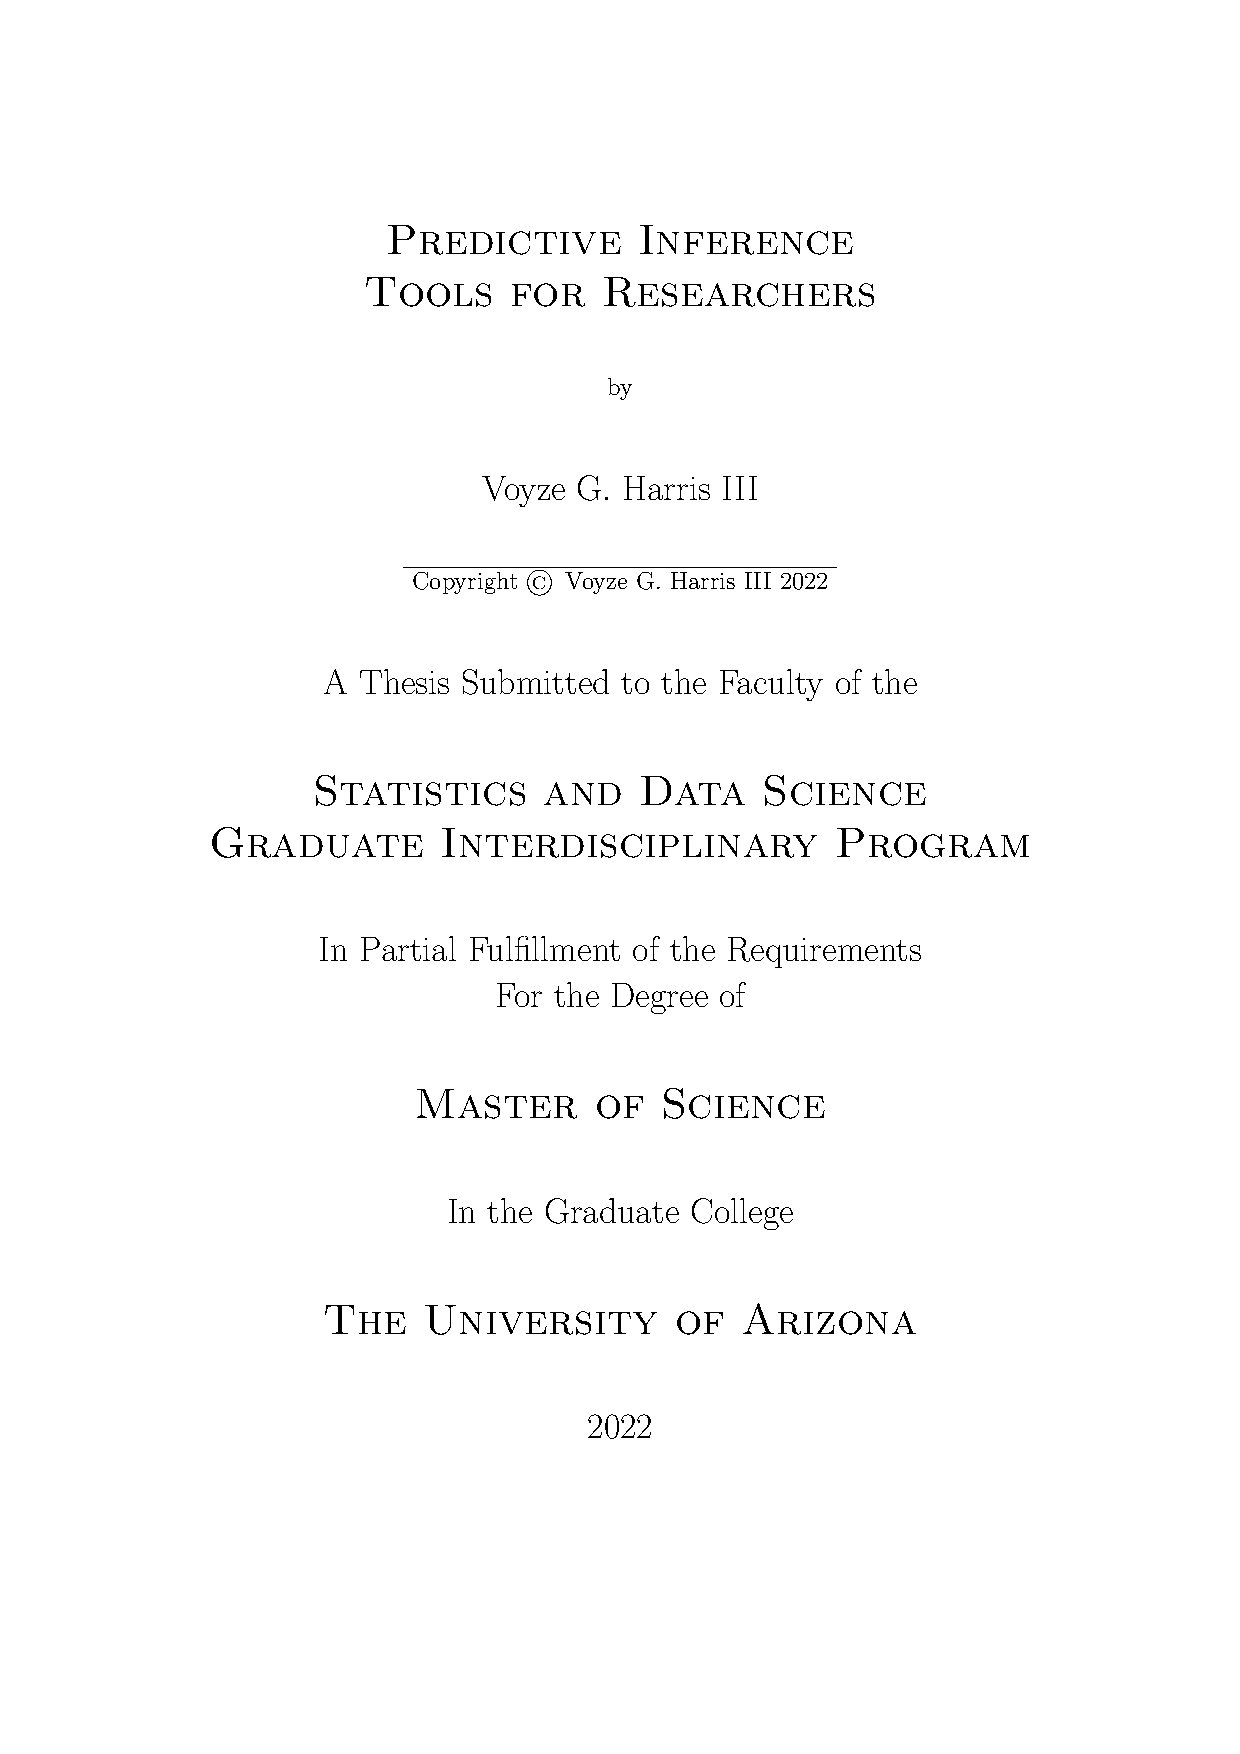
\includepdf{TitlePage_MastersThesis}

\includepdf{ThesisApprovalPage}
% \includepdf{Acknowledgements}



\noindent\begin{LARGE}\textbf{Acknowledgements}\end{LARGE}

\vspace{2cm}

\noindent This thesis is the culmination of an unusually long master’s program, which would not have been possible without the support of many people.

\vspace{1cm}

\noindent First I want to thank my thesis advisor, Dr. Dean Billheimer, for the many, many hours spent consulting, guiding, reading, and re-reading.  Also my committee members, Dr. Edward Bedrick and Dr. Walter Piegorsch, whose classes I survived, and who always encouraged me.

\vspace{1cm}

\noindent I also owe my thanks to the University of Arizona, the Math Department, and specifically the Statistics and Data Science Graduate Interdisciplinary program, for offering this course of study and allowing me to participate.

\vspace{1cm}

\noindent Thank you to my employer, Raytheon, who encourages ongoing growth and education, and makes it possible by means of flexible work scheduling, and by funding.  Thank you to my professional colleagues who rooted for me, especially John Rascon, Mitch Moffet, Dr. Kim Christianson, John Leach, Hahn Kim, Dr. Greg Paine, Dr. Dan Bentz, Dr. Kelly Villareal, Jimmy Parry, Ryan Ziegler, Ariel Boston, Chris Turner, Dr. Terrill Hurst, Dr. Al Mense, and Gary Garcia.

\vspace{1cm}

\noindent My dear friends Amy Duncan, Jenna Perryman, Dan Manship, Alex Swindle, and Danny Reckart showed me love and support I did not look for.

\vspace{1cm}

\noindent My sister, my parents, and my parents-in-law always cheer for me.

\vspace{1cm}

\noindent My wonderful children challenge and inspire me, and they rejuvenate me with their love and enthusiasm.

\vspace{1cm}

\noindent And finally, I don’t have words to express my deep gratitude to my beloved wife, Trish, who has endured my long hours and late nights for several years, who wants me in her life, and whose constant words of loving affirmation and sweet affection are a gift I can never repay.

\vspace{1cm}


\clearpage

\Sconcordance{concordance:Thesis_PostDefense_rev.tex:Thesis_PostDefense_rev.Rnw:%
1 71 1 1 0 51 1 1 4 92 1 1 81 197 1 1 62 100 1 1 18 15 1 1 58 189 1 1 %
55 152 1 1 118 91 1 1 39 13 1 1 43 98 1 1 39 15 1 1 25 27 1 1 71 87 1 1 %
14 28 1 1 33 12 1 1 22 130 1 1 51 26 1 1 110 640 1}


\tableofcontents
\listoffigures
\newpage


%%%%%%%%%%%%%%%%%%%%%%%%%%%%%%%%%
%%INTRODUCTION
%%%%%%%%%%%%%%%%%%%%%%%%%%%%%%%%%
\section{Abstract}
%% dean - I think you should include a bit more on predictive inferenc in the
%% abstract - add 2-3 sentences about how it's different from parametric
%% inference and why it's useful. You don't really need to much detail about the
%% function naming convention

An obstacle to widespread employment of Bayesian predictive inference in scientific research is the lack of suitable computing tools.  In this thesis I document several established useful models, and provide an applicable set of tools for statisticians.  For each of the included models, some basic notes on mathematical derivation are presented, and predictive inference is illustrated with examples.  For the details of the models and some of the examples I relied primarily on Seymour Geisser's \underline{Predictive Inference:  An Introduction} (1993) [3] and Peter D. Hoff's \underline{A First Course in Bayesian Statistical Methods} (2009) [5].\\

\noindent An R package has been developed, the main purpose of which is to provide the researcher with a means of generating samples from predictive distributions.  So for all the models, the package includes predictive sample generators.  For those models with analytical solutions, density and distribution functions are also provided.  The standard R naming convention for these function classes has been adopted:  density functions are prefixed with the letter ``d," distribution functions with the letter ``p," and sample generation functions with the letter ``r."  Also included in all function names is the abbreviation ``pred" (for predictive) and an initialism or abbreviation identifying the model itself.  For example, the density function for the Beta-Binomial model is named ``\texttt{dpredBB()}."  The R code for each function is included in the Appendix.


% \clearpage

\section{Introduction:  Predictive Inference}

My understanding of Bayesian Predictive Inference began with the University of Arizona course ``Bayesian Statistical Theory and Applications" under Dr. Edward Bedrick.  Since then it has been shaped by exposure to other sources, including various articles in academic journals, the aforementioned texts by Hoff and Geisser, and others including \underline{Bayesian Data Analysis} (2013) by Andrew Gelman, John B. Carlin, Hal S. Stern, David B. Dunson, Aki Vehtari, and Donald B. Rubin [4], \underline{Statistical Prediction Analysis} by J. Aitchison and I.R. Dunsmore [1], and excerpts from \underline{The Signal and the Noise} by Nate Silver [6].  In the next section and what follows, the ideas expressed are an amalgam of what was learned from this body of scholarship.

  \subsection{Why Predictive Inference?}


I find persuasive the assertion that the main purpose of statistics is to predict future events based on observed data, and moreover that a statistical model may be judged chiefly by the quality of its predictions.  Predictions about meaningful quantities that are relevant to the object of study facilitate scientific progress in multiple ways.  Nate Silver notes:

\begin{quote}
Prediction is important because it connects subjective and objective reality. Karl Popper, the philosopher of science, recognized this view. For Popper, a hypothesis was not scientific unless it was falsifiable—meaning that it could be tested in the real world by means of a prediction. [6]
\end{quote}

\noindent Billheimer emphasizes the improvement of scientific accuracy and reproducibility Bayesian prediction provides by ``shifting our focus from `finding differences' among hypothetical parameters to predicting observable events based on our current scientific understanding." [2] Focus on observed data enables corroboration or refutation of current hypotheses through future experimentation, and informs decision-making by summarizing quantities of direct interest to the researcher.  Bayesian predictive inference shifts the focus of statistical analysis from estimation of hypothetical parameters to statements about concrete observables.\\

\noindent It is not the intent of this thesis to suggest that parametric inference should be abandoned in statistical analyses.  Conventional statistical inference techniques are useful for summarizing information about large quantities of data in a small number of usable values (parameter estimates), and leveraging such summaries to determine whether a particular problem merits continued attention. Indeed, the scientific discipline of mathematical statistics has developed along parametric lines, imparting greater efficiency to the solving of idealized versions of problems. However, this focus on parameters has largely ignored the impact of observable quantities which may exhibit distributions very different from our (idealized) standard models. In support of prediction in general, and Bayesian prediction in particular, I return to Nate Silver :\\

\begin{quote}
Making predictions based on our beliefs is the best (and perhaps even the only) way to test ourselves. If objectivity is the concern for a greater truth beyond our personal circumstances, and prediction is the best way to examine how closely aligned our personal perceptions are with that greater truth, the most objective among us are those who make the most accurate predictions. Fisher’s statistical method, which saw objectivity as residing within the confines of a laboratory experiment, is less suitable to this task than Bayesian reasoning [6].
\end{quote}



\noindent Prediction is a means of discriminating between scientific hypotheses. Generally, a model may be judged by the quality of its predictions.  Given competing models, the better predictor will be given more weight, and a useful model increases in utility as its predictive capability improves.  With Bayesian inference, prior informed opinion about parameter distributions, updated with knowledge gained through observations, yields better predictions with each update.\\

% \setlength{\intextsep}{20pt}
% \begin{wrapfigure}{L}{0.35\textwidth}
%   \begin{center}
%     
\includegraphics[width=0.28\textwidth]{./Graphics/PassThePigs/PtPBox}
%   \end{center}
%   \caption{Pass The Pigs\textsuperscript{\circledR}}
% \end{wrapfigure}

\setlength{\intextsep}{20pt}
\begin{wrapfigure}{L}{0.35\textwidth}
  \centering
    
\includegraphics[width=0.28\textwidth]{./Graphics/PassThePigs/PtPBox}
  % \end{center}
  \caption{Pass The Pigs\textsuperscript{\circledR}}
\end{wrapfigure}

\noindent To illustrate the potential difference between Bayesian prediction and the use of plug-in estimators, consider the game Pass the Pigs\textsuperscript{\circledR}, a push-your-luck dice game in which the ``dice" are actually rubber pig figures.  Two pig dice are thrown, and points are scored according to the combination of positions in which they come to rest.  Details about the game can be found on Wikipedia here: \url{https://en.wikipedia.org/wiki/Pass_the_Pigs}\\

\noindent For the purpose of this example, consider the probability of a single pig landing in the ``Razorback" position, which occurs when the pig is lying on its back with its legs extended upward.  The irregular shape of the pig makes it difficult to assign probabilities to results other than by means of experimentation.  Such an experiment was conducted at Duquesne University, and an article describing the experiment as well as Bayesian predictive inference performed on the results appeared in the \textit{Journal of Statistics Education} Volume 14, Number 3, in 2006.  The article can be accessed here:  \url{http://jse.amstat.org/v14n3/datasets.kern.html}. Of the $11,954$ recorded results for individual pigs, approximately $22.4\%$ were Razorbacks.\\

\noindent Suppose in new data $t=4$ Razorbacks have been observed out of $N=10$ tosses of a single pig die, suggesting a straightforward binomial distribution with $\theta =$ Pr(Razorback) $= t/N = 0.4$. Taking the Duquesne experiment into consideration, we'll perform Bayesian prediction using various Beta prior distributions for $\theta$: $\theta\sim\text{Beta}(2,8)$, $\theta\sim\text{Beta}(22,78)$, and $\theta\sim\text{Beta}(224,776)$, and compare these results to predictions obtained from the plug-in estimator $\theta = 0.4$.   Any number of prior distributions on $\theta$ would satisfy the condition that $E(\theta) \approx 0.224$, suggested by the prior information.  The specific choice of a Beta prior is made largely for computational convenience.\\

\begin{wrapfigure}{r}{0.30\textwidth}
  \centering
    
\includegraphics[width=0.28\textwidth]{./Graphics/PassThePigs/Razorback}
  % \end{center}
  \caption{Razorback}
\end{wrapfigure}

\noindent The researcher wants to predict how many Razorbacks will result from some number $M$ of future pig die rolls.  In this example, $M=100$ was used.  The density curves in the plot below show the influence of the choice of prior parameters on the location and variance of the predictive distribution.  Essentially, each pair of shape parameters $(\alpha,\beta)$ in the Beta prior reflects the researcher's level of reliance on the results of the Duquesne experiment, with the ``weight" given to that knowledge increasing with the shape parameters by orders of magnitude.  The choice of parameters might be influenced by such things as pig tossing method (perhaps the researcher is throwing them by hand rather than dropping them by the carefully controlled method used in the Duquesne experiment), or by a need to account for pig-to-pig variation, or anything else the researcher believes introduces a deviation from the events upon which the prior information is based.  Use of the scaled-up Big Pigs\texttrademark  variant, for example might give reason to use a very low-weighted prior such as $\theta\sim\text{Beta}(2,8)$.\\

\noindent Figure \ref{fig:PtPBB} and the table below illustrate the effects of the Bayesian prediction method. Perhaps most notable is the location disparity between the plug-in (Binomial) prediction and the family of Bayesian (Beta-binomial) predictive distributions.  The consideration of prior knowledge is also shown to have a significant effect.  In this example, the strong influence of the choice of shape parameters for the Beta prior on the mean and variance of the predictive distribution provides options for the future prognosticator. If a new set of trials closely duplicates the Duquesne experimental conditions, for example, predictions might be based on the result from the Beta$(224,776)$ prior.  A lower-weighted prior might be used for any experimental element the researcher believes introduces a deviation from the knowledge upon which the prior information is based.

\begin{figure}[h]
  \centering
  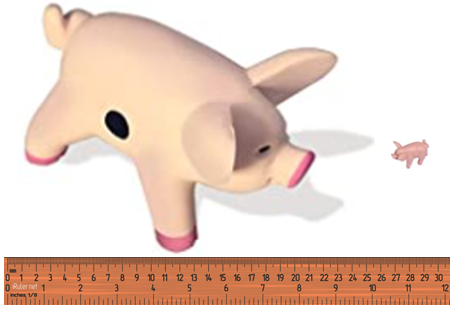
\includegraphics[width=0.9\textwidth]{./Graphics/PassThePigs/PigSize_wRuler}
  \caption{Big Pigs\texttrademark to Original (Approximate Scale)}
\end{figure}


\vspace{1cm}

\begin{figure}[ht]
  \centering
  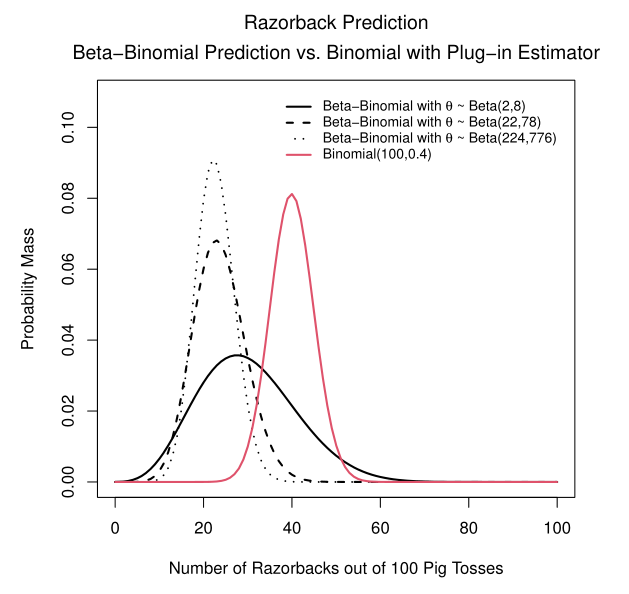
\includegraphics[width=0.8\textwidth]{./Graphics/PassThePigs/PTP_BBplot}
  \caption{Pass the Pigs\textsuperscript{\circledR} Prediction}
  \label{fig:PtPBB}
\end{figure}

\vspace{2cm}


\vspace{1cm}

\begin{center}
  \begin{tabular}{l c c c c }
  \toprule
  \multicolumn{5}{c}{\large \#Razorbacks Predicted out of 100 Tosses}          \\
  \multicolumn{1}{c}{\textbf{Prediction Method}} & \multicolumn{1}{c}{$\textbf{(}\boldsymbol\alpha,\boldsymbol\beta\textbf{)}$}  & \multicolumn{1}{c}{\textbf{Prior Mean }$\textbf{E(}\boldsymbol\theta\textbf{)}$}  & \multicolumn{1}{c}{\textbf{Prediction Mean}} & \multicolumn{1}{c}{\textbf{SD}}\\
        \midrule
        Beta-Binomial & (2,8) & 0.2 & 30.03 & 11.06 \\
        \midrule
        Beta-Binomial & (22,78) & 0.22 & 23.32 & 5.7\\
        \midrule
        Beta-Binomial & (224,776) & 0.224 & 22.47 & 4.36 \\
        \midrule
        Binomial$(100,0.4)$ & -- & -- & 40 & 4.9 \\
  \bottomrule
  \end{tabular}
\end{center}

% \vspace{1cm}

\noindent The differences in the results of the two prediction methods are easy to see in this case. Unlike the Bayesian approach, the binomial-only model uses only the observed data, does not account for any uncertainty in the binomial parameter ($\theta$), and ignores historical info about Razorback frequency.  If speculating whether the number of razorbacks out of the next 10 pig tosses will be greater than, say, 3, the indications of the two analysis approaches contradict each other.  The statistically savvy wagerer of course realizes that the 10 die throws informing the plug-in results do not offer high predictive confidence.  A much less risky option for the bettor is the Bayesian method with a suitable prior parameterization.


\clearpage

  \subsection{The Bayesian Parametric Prediction Format}

\noindent We want to predict future outcomes based on current knowledge.
Specifically we're asking: for observed values $Y_1 = y_1,...,Y_n = y_n$, what
is likely to be the value of the next observation, $\tilde{Y}$?  We want to compute $Pr(\tilde{Y}|y_1,...,y_n)$, where $y_1,...,y_n$ are
conditionally independent and identically distributed (i.i.d.) with respect to  a population parameter (or parameters) $\theta$.  We assign prior distribution
 $\pi(\theta)$ based on some existing knowledge or beliefs.  Here we are careful to satisfy ourselves that $Y_1,...,Y_n$ are \textit{exchangeable}, which
 enables us to rely on de Finetti's representation theorem for the conditional independence assumption.  Exchangeability means essentially that the order of the observations conveys no information affecting the distribution of the data.  That is, $p(Y_1,...,Y_n) = p(Y_{\pi_1},...,Y_{\pi_n})$ for any permutation $\pi_1,...,\pi_n$ of the indices $1,...,n$.\\

\begin{quote}
  \textbf{De Finetti's Theorem:  } Let $Y_i\in\mathcal{Y}$ for all $i\in\{1,2,...\}$.  Suppose that, for any $n$, our belief model for $Y_1,...,Y_n$ is exchangeable. Then our model can be written as

  $$p(y_1,...,y_n) = \int\left\{\prod_1^n p(y_i|\theta)\right\}p(\theta)d\theta$$

  for some parameter $\theta$, some prior distribution on $\theta$ and some sampling model $p(y|\theta)$.  The prior and sampling model depend on the form of the belief model $p(y_1,...,y_n)$.\\
\end{quote}

\noindent Simply put, exchangeability of data implies (conditional) independence and identical distribution (i.i.d.) with respect to a parameter with some prior distribution. The converse is immediate from the definition of marginal probability and the commutative property of multiplication. Hoff [5] summarizes these ideas like this (p. 29):\\


\[
\begin{rcases}
Y_1,...,Y_n|\theta \text{ are i.i.d}\\
\theta\sim\pi(\theta)
\end{rcases} \Leftrightarrow Y_1,...,Y_n \text{ are exchangeable for all } n
\]

\vspace{5mm}

\noindent The derivations throughout this thesis assume exchangeability, so we can formulate predictive probability as follows:

% \begin{flalign}
%   p(\tilde{Y} = \tilde{y} | Y_1 = y_1,...,Y_n = y_n) &= \frac{p(\tilde{y},y_1,...,y_n)}{p(y_1,...,y_n)}\nonumber\\
%   &\nonumber\\
%   &=\frac{\int p(\tilde{y},y_1,...,y_n | \theta)\pi(\theta) d\theta}{p(y_1,...,y_n)}\nonumber\\
%   &\nonumber\\
%   &= \frac{\int p(\tilde{y}|\theta)p(y_1,...,y_n | \theta)\pi(\theta) d\theta}{p(y_1,...,y_n)}\nonumber\\
%   &\nonumber\\
%   &= \frac{\int p(\tilde{y}|\theta)p(\theta|y_1,...,y_n) p(y_1,...,y_n) d\theta}{p(y_1,...,y_n)}\nonumber\\
%   &\nonumber\\
%   &= \int p(\tilde{y}|\theta) p(\theta|y_1,...,y_n) d\theta \label{BayesianPredictiveFormat}
% \end{flalign}


\begin{flalign}
  p(\tilde{y} | y_1,...,y_n) &= \frac{p(\tilde{y},y_1,...,y_n)}{p(y_1,...,y_n)}\nonumber\\
  &\nonumber\\
  &=\frac{\int p(\tilde{y},y_1,...,y_n | \theta)\pi(\theta) d\theta}{p(y_1,...,y_n)}\nonumber\\
  &\nonumber\\
  &= \frac{\int p(\tilde{y}|\theta)p(y_1,...,y_n | \theta)\pi(\theta) d\theta}{p(y_1,...,y_n)}\nonumber\\
  &\nonumber\\
  &= \frac{\int p(\tilde{y}|\theta)p(\theta|y_1,...,y_n) p(y_1,...,y_n) d\theta}{p(y_1,...,y_n)}\nonumber\\
  &\nonumber\\
  &= \int p(\tilde{y}|\theta) p(\theta|y_1,...,y_n) d\theta \label{BayesianPredictiveFormat}
\end{flalign}

\noindent For prediction, we need only to characterize the observed data $(y_1,...,y_n)$, conditionally independent with respect to  $\theta$, and supply a suitable prior distribution $\pi(\theta)$.  Then we compute posterior $p(\theta|y) = p(y|\theta)\pi(\theta)/\int_\theta p(\theta)p(y|\theta)d\theta$ and generate the predictive distribution using   (\ref{BayesianPredictiveFormat}).  In some cases the integral has an analytical solution, while in others we evaluate it through Monte Carlo (MC) sampling. Note that the predictive distribution is completely specified, with no unknowns.



\clearpage

\section{Predictive Problems with Conjugate Priors}

\noindent When data can be modeled with a distribution that suggests a conjugate prior for the parameter(s) of interest, and those parameters can reasonably be represented by that conjugate prior, the posterior calculations are greatly simplified.  The four classes of models addressed in this section all exhibit this feature.  The first three are single-parameter exponential families and have closed-form solutions for prediction.  The fourth is a two-parameter exponential family with unkown mean and variance.  While this one does not admit an analytical solution, prediction is easily accomplished by means of simple Monte Carlo sampling.  The four classes of predictive models presented in this section are:
\begin{itemize}
  \item Beta-Binomial ($T = \sum Y\sim$ Binom$(N,\theta)$ with $\theta\sim$ Beta)
  \item Exponential-Gamma ($Y\sim$ Exp$(\theta)$ data with $\theta\sim$ Gamma)
  \item Poisson-Gamma ($Y\sim$ Poi$(\theta)$ data $\theta\sim$Gamma)
  \item Normal-Inverse Gamma ($Y\sim$ Normal$(\theta,\sigma)$ data with $\theta\sim$ Normal and $\sigma\sim$ Inverse Gamma)
\end{itemize}

\noindent Throughout this section, $N$ is used for the observed data sample
size, and $S$ is the size of the desired predictive sample. The predicted future result
is indicated by surmounting the variable name with a tilde.  For example, when the observed data is represented by $y$, the prediction is designated $\tilde{y}$. Parameter names are clearly indicated as they appear.

  \subsection{Prediction of Future Successes:  Beta-Binomial [3]}


    \subsubsection{Derivation (Beta-Binomial)}

    \noindent Let $Y_1,...,Y_N$ be exchangeable binary variables, and therefore conditionally i.i.d.  with respect to some parameter $\theta$, $\theta\in[0,1]$. That is, Pr$(Y_i = 1|\theta) = \theta$, with $Y_i = 1$ indicating success and $Y_i = 0$ indicating failure.  The number of observed successes can be represented by $T = \sum Y_i$, which is sufficient for $\theta$ and has a binomial$(N,\theta)$ distribution.  That is,

      $$Pr(T = t|\theta) = {N\choose t}\theta^t(1-\theta)^{N-t}.$$

      \vspace{5mm}

\noindent Assuming $\theta\sim\text{Beta}(\alpha,\boldsymbol\beta)$, we have prior distribution

      \vspace{5mm}

      $$\pi(\theta) = \frac{\Gamma(\alpha + \beta)\theta^{\alpha - 1}(1 - \theta)^{\beta - 1}}{\Gamma(\alpha)\Gamma(\beta)} \text{ with } \alpha, \beta > 0$$

      \vspace{5mm}

\noindent The posterior distribution of $\theta$ given $Y_1,...,Y_N$, then, is

      \vspace{5mm}


\begin{flalign*}
  p(\theta|Y_1,...,Y_N) = p(\theta|t) &= \frac{p(t|\theta)\pi(\theta)}{\int p(t|\theta)\pi(\theta)d\theta}\\
  &\\
  &= \frac{{N\choose t}\theta^t(1-\theta)^{N-t}\frac{\Gamma(\alpha + \beta)\theta^{\alpha - 1}(1 - \theta)^{\beta - 1}}{\Gamma(\alpha)\Gamma(\beta)}}{\int{N\choose t}\theta^t(1-\theta)^{N-t}\frac{\Gamma(\alpha + \beta)\theta^{\alpha - 1}(1 - \theta)^{\beta - 1}}{\Gamma(\alpha)\Gamma(\beta)}d\theta}\\
  &\\
  &= \frac{\theta^{t+\alpha-1}(1-\theta)^{N-t+\beta-1}}{\int \theta^{t+\alpha-1}(1-\theta)^{N-t+\beta-1}d\theta}\\
  &\\
  &= \frac{\Gamma(N+\alpha+\beta)}{\Gamma(t+\alpha)\Gamma(N-t+\beta)}\theta^{t+\alpha-1}(1-\theta)^{N-t+\beta-1}\\
  &\\
  &= \text{Beta}(t+\alpha,N-t+\beta)
\end{flalign*}

\noindent Note that the ratio of Gamma functions in the final step appears as a scaling constant that enables the Beta$(t+\alpha,N-t+\beta)$ density function under the integrand in the denominator of the previous step to resolve to 1.

      \vspace{5mm}

      \noindent We want to predict the number $\tilde{T}$ of successes in a future experiment involving $M$ binary observations.  That is, $\tilde{T} = \sum_{i=1}^M Y_{N+i}$, and we have Beta-Binomial predictive distribution

\begin{flalign}
  \text{Pr}[\tilde{T} = \tilde{t}|T=t]
  &= \int p(\tilde{T} = \tilde{t}|\theta)p(\theta|t)d\theta\nonumber\\
  &\nonumber\\
  &= \int {M\choose \tilde{t}}\theta^{\tilde{t}}(1-\theta)^{M-\tilde{t}}\frac{\Gamma(N+\alpha+\beta)}{\Gamma(t+\alpha)\Gamma(N-t+\beta)}\theta^{t+\alpha-1}(1-\theta)^{N-t+\beta-1}d\theta\nonumber\\
  &\nonumber\\
  &= \frac{M!}{\tilde{t}!(M-\tilde{t})!}\frac{\Gamma(N+\alpha+\beta)}{\Gamma(t+\alpha)\Gamma(N-t+\beta)}\int\theta^{\tilde{t}+t+\alpha-1}(1-\theta)^{M+N-\tilde{t}-t+\beta-1}d\theta\nonumber  \\
  &\nonumber\\
  &= \frac{\Gamma(M+1)\Gamma(N+\alpha+\beta)\Gamma(\tilde{t}+t+\alpha)\Gamma(M+N-\tilde{t}-t+\beta)}{\Gamma(\tilde{t}+1)\Gamma(M-\tilde{t}+1)\Gamma(t+\alpha)\Gamma(N-t+\beta)\Gamma(M+N+\alpha+\beta)},\label{betaBinomial_pred}
\end{flalign}

\noindent an impressive combination of Gamma functions.  Note that the last two factors in the numerator together with the final factor in the denominator comprise the reciprocal of the scale factor corresponding with the Beta$(\tilde{t}+t+\alpha,M+N-\tilde{t}-t+\beta)$ kernel in the integrand, enabling the integral to resolve to 1.


% \clearpage

    \subsubsection{R Implementation (Beta-Binomial)}\label{sec:BBimp}

This result has been used to create R functions \texttt{dpredBB()}, \texttt{ppredBB()}, and \texttt{rpredBB()} for the Beta-Binomial predictive distribution for density, cumulative probability, and predictive sampling, respectively (see appendix for the R code).  The density function \texttt{dpredBB()} relies on the R function \texttt{lgamma()} to evaluate the numerator and denominator of the predictive distribution (\ref{betaBinomial_pred}) factor by factor logarithmically, and then exponentiates for the final result, evaluated at the desired integer value (or vector of values) $\tilde{y}$ input by the user.  The cdf \texttt{ppredBB()} simply calls \texttt{dpredBB()} and returns the cumulative sum of that discrete set of results.  The predictive sampler \texttt{rpredBB()} makes use of the inverse transform method and the output from the cdf \texttt{ppredBB()}.  Calls to these functions appear as follows:

\begin{center}
  \texttt{\hyperref[sec:dpredBB]{dpredBB(tpred,N,t,M,a,b)}}\\
  \texttt{\hyperref[sec:ppredBB]{ppredBB(tpred,N,t,M,a,b)}}\\
  \texttt{\hyperref[sec:rpredBB]{rpredBB(S,N,t,M,a,b)}}\\
\end{center}

\noindent where

\begin{flalign*}
  \texttt{tpred} &= \tilde{t} \text{, the number (or vector of numbers) of successes in a future experiment }\\
  &\text{ involving } M \text{ binary observations} \\
  \texttt{N} &= \text{the number of observations in the current data set}\\
  \texttt{t} &= \text{the number of successes out of the N observations in the current data set}\\
  \texttt{M} &= \text{the number of binary observations in a future experiment}\\
  \texttt{a} &= \alpha \text{, the first shape parameter of the Beta prior}\\
  \texttt{b} &= \beta \text{, the second shape parameter of the Beta prior}\\
  \texttt{S} &= \text{the desired predictive sample size; that is, the number of future experiments }\\
  &\text{ of size } M \text{ for which a predicted number of successes is desired}\\
\end{flalign*}

    \subsubsection{Example (Beta-Binomial)}

The functions \texttt{dpredBB()} and \texttt{rpredBB()} were used in the Pass The Pigs\textsuperscript{\circledR} example in the introduction.  Here, all three functions are exercised in an imagined experiment using the Big Pigs\texttrademark  variant.  Suppose $t=7$ Razorbacks have been observed out of $n=10$ tosses of Big Pigs\texttrademark, and the researcher has settled on prior distribution Pr(Razorback) = $\theta\sim\text{Beta}(2,8)$.  For $M = 10$ future observations, how many successes are predicted?  Figure \ref{fig:BBdist} below shows the predictive distribution from \texttt{dpredBB()}, the cumulative distribution from \texttt{ppredBB()}, and a histogram of 1000 draws from \texttt{rpredBB()}.

\begin{figure}[ht]
  \centering
  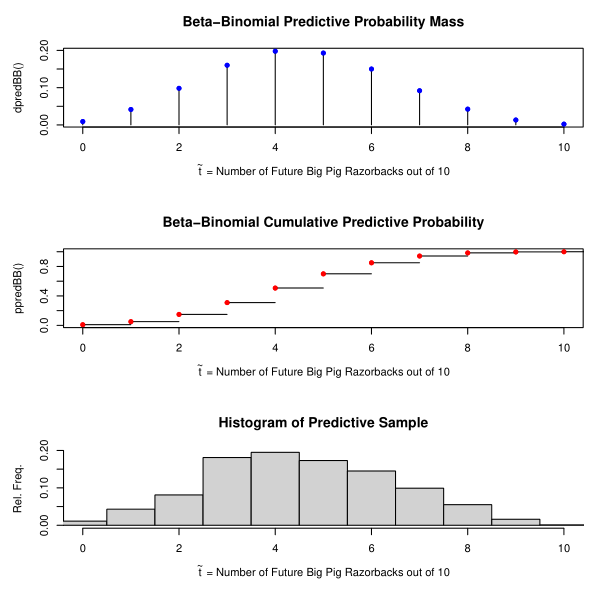
\includegraphics[width=0.95\textwidth]{./Graphics/DistributionPlots/BetaBinomial}
  \caption{Beta-Binomial Predictive Distribution}
  \label{fig:BBdist}
\end{figure}

\vspace{2cm}




    \subsection{Survival Time:  Exponential-Gamma [3]}

    \subsubsection{Derivation (Exponential-Gamma)}

Suppose $y_1,...,y_d$ represent fully observed realizations from an exponential survival time density
          $$p(y|\theta) = \theta e^{-\theta y}, y \geq 0, \theta > 0$$
      and $y_{d+1},...,y_N$ are the censoring time assigned to subjects surviving beyond the experimental time limit.  We assume $Y_1,...,Y_d$ are exchangeable and therefore conditionally i.i.d. with respect to $\theta$.\\

\noindent The usual exponential likelihood is used for the fully observed events, whereas for the censored subjects we need Pr$(Y > y | \theta) = 1 - \text{Pr}(Y\leq y | \theta) = 1 - F(y|\theta) = 1 - (1 - e^{-\theta y}) = e^{-\theta y}$.  Here $F$ denotes the cumulative distribution function.\\

\noindent Thus, with $\bar{y} = \frac{1}{N}\sum_{i=1}^N y_i$, the overall likelihood is

      $$L(\theta|y) = \prod_{i=1}^d\theta e^{-\theta y_i}\prod_{i=d+1}^N e^{-\theta y_i} = \theta^d e^{-\theta N\bar{y}}$$

\noindent Assuming a Gamma$(\delta,\gamma)$ prior for $\theta$,

       $$\pi(\theta) = \frac{\gamma^\delta\theta^{\delta - 1}e^{-\gamma\theta}}{\Gamma(\delta)} \text{ with } \delta, \gamma > 0$$

\noindent we obtain the posterior

        \begin{flalign*}
          p(\theta|y_1,...,y_N)
          &= \frac{p(y_1,...,y_N|\theta)\pi(\theta)}{\int p(y_1,...,y_N|\theta)\pi(\theta)d\theta}\\
          &\\
          &= \frac{\theta^d e^{-\theta N\bar{y}}\cdot\frac{\gamma^\delta\theta^{\delta - 1}e^{-\gamma\theta}}{\Gamma(\delta)}}{\int\left(\theta^d e^{-\theta N\bar{y}}\cdot\frac{\gamma^\delta\theta^{\delta - 1}e^{-\gamma\theta}}{\Gamma(\delta)}\right)d\theta}\\
          &\\
          &= \frac{\left(\theta^{d+\delta - 1}e^{-\theta(\gamma+N\bar{y})}\right)}{\int\left(\theta^{d+\delta - 1}e^{-\theta(\gamma+N\bar{y})}\right)d\theta}\\
          &\\
          &= \frac{(\gamma+N\bar{y})^{d+\delta}}{\Gamma(d+\delta)}\theta^{d+\delta - 1}e^{-\theta(\gamma+N\bar{y})}\\
          &\\
          &=\text{Gamma}(d+\delta,\gamma+N\bar{y}),
        \end{flalign*}

\noindent with the Gamma$(d+\delta,\gamma+N\bar{y})$ density in the denominator of next to last step integrating to $1$.\\

\noindent The survival time predictive probability density then is

    \begin{flalign}
      p(\tilde{Y}|y_1,...,y_N)
      &= \int p(\tilde{y}|\theta)p(\theta|y_1,...,y_N)d\theta\nonumber\\
      &\nonumber\\
      &= \int \theta e^{-\theta \tilde{y}} \cdot \frac{(\gamma+N\bar{y})^{d+\delta}\theta^{d+\delta - 1}e^{-\theta(\gamma+N\bar{y})}}{\Gamma(d+\delta)}d\theta\nonumber\\
      &\nonumber\\
      &= (d+\delta)(\gamma+N\bar{y})^{d+\delta}\int\frac{\theta^{(d+\delta + 1) - 1}e^{-\theta(\gamma+N\bar{y} + \tilde{y})}}{(d+\delta)\Gamma(d+\delta)}d\theta\nonumber\\
      &\nonumber\\
      &= \frac{(d+\delta)(\gamma+N\bar{y})^{d+\delta}}{\left(\gamma+N\bar{y}+\tilde{y}\right)^{d+\delta+1}}\int\frac{\left(\gamma+N\bar{y}+\tilde{y}\right)^{d+\delta+1}\theta^{(d+\delta + 1) - 1}e^{-\theta(\gamma+N\bar{y} + \tilde{y})}}{\Gamma(d+\delta+1)}d\theta\nonumber\\
      &\nonumber\\
      &= \frac{(d+\delta)(\gamma+N\bar{y})^{d+\delta}}{\left(\gamma+N\bar{y}+\tilde{y}\right)^{d+\delta+1}}\label{exponentialGamma_pred},
    \end{flalign}

\noindent simplifying here by constructing a Gamma$(d+\delta+1,\gamma+N\bar{y}+\tilde{y})$ density in the final integrand.\\



    \subsubsection{R Implementation (Exponential-Gamma)}\label{sec:EGimp}

This result has been used to create R functions \texttt{dpredEG()}, \texttt{ppredEG()}, and \texttt{rpredEG()} for the Gamma-Exponential distribution for density, cumulative probability, and predictive sampling, respectively (see appendix for R code).  These functions are exercised in the following example. \\

\noindent The density function \texttt{dpredEG()} evaluates the numerator and denominator of the predictive density logarithmically (using the R function \texttt{log()}) and then exponentiates to produce the result.  The cdf \texttt{ppredEG()} integrates the pdf at each discrete value using the R function \texttt{integrate()}.  The predictive sampler \texttt{rpredEG()} draws posterior $\theta|y_1,...,y_i\sim\text{Gamma}(d+\delta,\gamma+\sum y_i)$ and then draws predictions from Exp$(\theta)$. Calls to these functions appear as follows:

\begin{center}
  \texttt{\hyperref[sec:dpredEG]{dpredEG(ypred,y,c,dt,gm)}}\\
  \texttt{\hyperref[sec:ppredEG]{ppredEG(ypred,y,c,dt,gm)}}\\
  \texttt{\hyperref[sec:rpredEG]{rpredEG(S,y,c,dt,gm)}}\\
\end{center}

\noindent where

\begin{flalign*}
  \texttt{ypred} &= \tilde{y} \text{, the event time(s) in future experiments for which prediction is desired}\\
  \texttt{y} &= \text{a vector of } N \text{ event times, } d \text{ observed, } N-d \text{ censored}\\
\end{flalign*}

\begin{flalign*}
  \texttt{c} &= \text{an indicator vector of length } N.\texttt{  c[i]=1}\text{ if the corresponding data element }\texttt{y[i]}\text{ is fully }\\ &\text{   observed, otherwise }\texttt{c[i]=0.}  \text{  Note }\texttt{d = sum(c).}\\
  \texttt{dt} &= \delta \text{, the shape parameter of the Gamma prior}\\
  \texttt{gm} &= \gamma \text{, the rate parameter of the Gamma prior}\\
  \texttt{S} &= S \text{, the sample size to be generated by the predictive distribution}\\
\end{flalign*}


%%%%%%%%%%%%%%%%%%%%%%%%%%%
%%%%%%%%%%%%%%%%%%%%%%%%%%%


    \subsubsection{Example (Exponential-Gamma)}

\noindent Aitchison and Dunsmore [1] provide survival time data representing the lifetime in minutes of 24 machine tools of a particular type. Inspection and replacement costs depend on the machines' lifespans, so reliable predictions are financially relevant to the factory in which the machines are used. The observed machine lifetimes range from 4 to 290, with mean 74.71.  For this example, we'll assume the observations were censored at three hours, that is, censoring time $t_c = 180$ minutes.  The data set includes three survival times that exceed 180 minutes, so to construct our example we replace those with the censoring time, and the mean is reduced to 72.21.  The data are plotted in Figure \ref{fig:EG_Data} with the three censored values shown in red.  The gray horizontal line depicts the average (after censoring).

\begin{figure}[h]
  \centering
  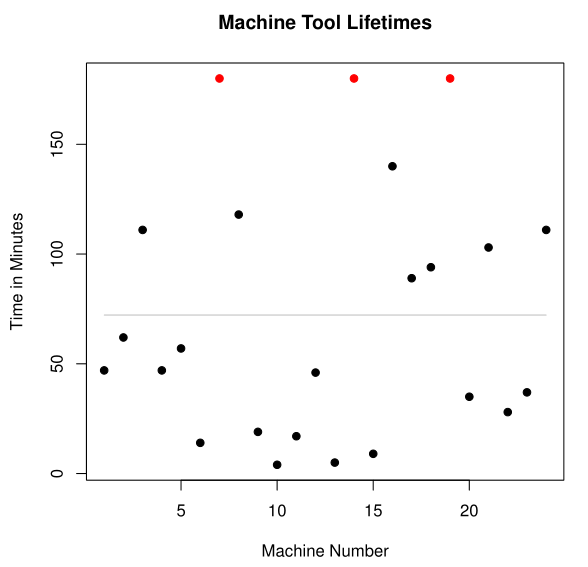
\includegraphics[width=0.7\textwidth]{./Graphics/ExamplePlots/EG_TimeData}
  \caption{Observed Machine Tool Lifetime Data}
  \label{fig:EG_Data}
\end{figure}

\vspace{2cm}


\noindent We will assume the data are distributed exponentially with respect to some parameter $\theta$.  Suppose prior knowledge suggests that the average survival time is around 80 minutes.  In terms of the exponential distribution then $E(y) = 1/\theta \approx 80$.  For the Gamma$(\delta,\gamma)$ prior, parameter values of $\delta = 0.5$ and $\gamma=50$ were chosen. These values correspond with a median Exponential parameter value of $1/80$ and assign about a 20\% probability to values of $\theta$ less than $1/120$. Figure \ref{fig:EGdist} below illustrates the predictive probability using \texttt{dpredEG()} and \texttt{rpredEG()}, along with a histogram of a predictive sample of size 1000 returned by \texttt{rpredEG()}.\\

\noindent Under the assumptions of this model the mean of the predictive sample (86.85) is somewhat larger than that of the observed data, and this information will likely influence the factory budget.


\begin{figure}[ht]
  \centering
  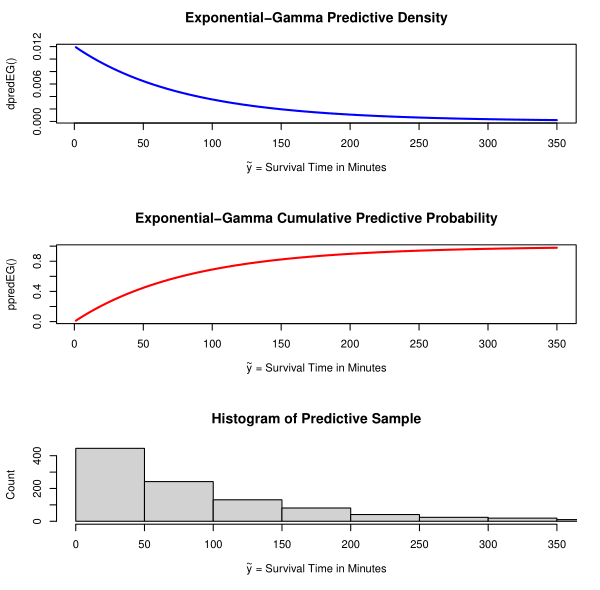
\includegraphics[width=0.95\textwidth]{./Graphics/DistributionPlots/ExponentialGamma}
  \caption{Exponential-Gamma Predictive Distribution}
  \label{fig:EGdist}
\end{figure}

\vspace{2cm}





%%%%%%%%%%%%%%%%%%%%%%%%%%%%%%
%%%%%%%%%%%%%%%%%%%%%%%%%%%%%%

\clearpage

  \subsection{Poisson-Gamma Model [5]}

    \subsubsection{Derivation (Poisson-Gamma)}

      Suppose we have exchangeable count data observations $Y_1,...,Y_N|\theta\overset{i.i.d.}{\sim}\text{Poisson}(\theta)$, with $\theta$ assumed to have prior Gamma$(\alpha,\beta)$ distribution.  That is,

      \begin{flalign*}
        P\left(Y_1 = y_1,...,Y_N = y_N|\theta\right)
        &= \prod_{i=1}^N p\left(y_i|\theta\right)\\
        &\\
        &= \prod_{i=1}^N\frac{1}{y_i!}\theta^{y_i}e^{-\theta}\\
        &\\
        &= \left(\prod_{i=1}^N\frac{1}{y_i!}\right)\theta^{\sum y_i}e^{-N\theta}\\
        &\\
        &= c\left(y_1,...,y_N\right)\theta^{\sum y_i}e^{-N\theta}, y_i\in\{0,1,2,...\}, \theta > 0
      \end{flalign*}

\noindent and

      $$\pi(\theta) = \dfrac{\beta^\alpha}{\Gamma(\alpha)}\theta^{\alpha-1}e^{-\beta\theta} \text{ with } \alpha, \beta > 0.$$

\bigskip

\noindent Then we have posterior

      \begin{flalign*}
        p\left(\theta|y_1,...,y_N\right)
        &= \dfrac{p\left(y_1,...,y_N|\theta\right)\pi(\theta)}{\int_\theta p\left(y_1,...,y_N|\theta\right)p(\theta)d\theta}\\
        &\\
        &= \dfrac{p\left(y_1,...,y_N|\theta\right)\pi(\theta)}{p\left(y_1,...,y_N\right)}\\
        &\\
        &= \dfrac{1}{p\left(y_1,...,y_N\right)}\theta^{\sum y_i}e^{-N\theta}\dfrac{\beta^\alpha}{\Gamma(\alpha)}\theta^{\alpha - 1}e^{-\beta\theta}\\
        &\\
        &= C\left(y_1,...,y_N,\alpha,\beta\right)\theta^{\alpha+\sum y_i - 1}e^{-(\beta + N)\theta}\\
        &\\
        &\propto \text{Gamma}\left(\alpha+\sum y_i,\beta + N\right).
      \end{flalign*}

\noindent Here

      \begin{flalign*}
        C\left(y_1,...,y_N,\alpha,\beta\right)
        &= \dfrac{1}{p\left(y_1,...,y_N\right)}\cdot\dfrac{\beta^\alpha}{\Gamma(\alpha)}\\
        &\\
        &= \dfrac{1}{\int_\theta p\left(y_1,...,y_N|\theta\right)\pi(\theta)d\theta}\cdot\dfrac{\beta^\alpha}{\Gamma(\alpha)}\\
        &\\
        &= \dfrac{1}{\int_\theta\left(\prod\frac{1}{y_i!}\right)\theta^{\sum y_i}e^{-N\theta}\cancel{\left(\frac{\beta^\alpha}{\Gamma(\alpha)}\right)}\theta^{\alpha-1}e^{-\beta\theta}d\theta}\cdot\cancel{\left(\frac{\beta^\alpha}{\Gamma(\alpha)}\right)}
        &\\
        &= \dfrac{1}{\left(\prod\frac{1}{y_i!}\right)\frac{\Gamma(\alpha + \sum y_i)}{(\beta+N)^{\alpha+\sum y_i}}\int_\theta \frac{(\beta+N)^{\alpha+\sum y_i}}{\Gamma(\alpha+\sum y_i)}\theta^{\sum y_i+\alpha-1}e^{-(\beta+N)\theta}d\theta}\\
        &\\
        &= \dfrac{\prod_{i=1}^N y_i!(\beta+N)^{\alpha+\sum y_i}}{\Gamma(\alpha+\sum y_i)}
      \end{flalign*}

\noindent Call this constant $C_N$ (for $N$ observations).

\bigskip

\noindent Note that with an additional observation $\tilde{y} = y_{N+1}$ the constant becomes

      $$C_{N+1} = \dfrac{\prod_{i=1}^{N+1} y_i!(\beta+N+1)^{\alpha+\sum_{i=1}^{N+1} y_i}}{\Gamma(\alpha+\sum_{i=1}^{N+1} y_i)}.$$

\noindent Also note that the marginal joint distribution of $k$ observations is

      $$p(y_1,...,y_k) = \dfrac{1}{C_k}\dfrac{\beta^\alpha}{\Gamma(\alpha)}.$$

\noindent For future observation $\tilde{y}$, then, we compute predictive distribution

      \begin{flalign}
        p\left(\tilde{Y}|y_1,...,y_N\right)
        &= \dfrac{p\left(y_1,...,y_N,\tilde{y}\right)}{p\left(y_1,...,y_N\right)} = \dfrac{p\left(y_1,...,y_{N+1}\right)}{p\left(y_1,...,y_N\right)}
        = \dfrac{\frac{1}{C_{N+1}}\cancel{\frac{\beta^\alpha}{\Gamma(\alpha)}}}{\frac{1}{C_N}\cancel{\frac{\beta^\alpha}{\Gamma(\alpha)}}}
        = \dfrac{C_N}{C_{N+1}}\nonumber\\
        &\nonumber\\
        &= \dfrac{\dfrac{\prod_{i=1}^N y_i!(\beta+N)^{\alpha+\sum_{i=1}^N y_i}}{\Gamma(\alpha+\sum_{i=1}^N y_i)}}{\dfrac{\prod_{i=1}^{N+1} y_i!(\beta+N+1)^{\alpha+\sum_{i=1}^{N+1} y_i}}{\Gamma(\alpha+\sum_{i=1}^{N+1} y_i)}}\nonumber
      \end{flalign}
      \begin{flalign}
        \,\,\,\,\,\,\,&= \dfrac{\Gamma\left(\alpha+\sum_{i=1}^{N+1}y_i\right)(\beta+N)^{\alpha+\sum_{i=1}^N y_i}}{\left(y_{N+1}!\right)\Gamma\left(\alpha+\sum_{i=1}^N y_i\right)(\beta+N+1)^{\alpha+\sum_{i=1}^{N+1}y_i}}\nonumber\\
        &\nonumber\\
        &= \dfrac{\Gamma\left(\alpha+\sum_{i=1}^N y_i + \tilde{y}\right)(\beta+N)^{\alpha+\sum_{i=1}^N y_i}}{\left(\tilde{y}!\right)\Gamma\left(\alpha+\sum_{i=1}^N y_i\right)(\beta+N+1)^{\alpha+\sum_{i=1}^N y_i + \tilde{y}}}\nonumber\\
        &\nonumber\\
        &= \dfrac{\Gamma\left(\alpha+\sum y_i+\tilde{y}\right)}{\Gamma(\tilde{y}+1)\Gamma(\alpha+\sum y_i)}\cdot \left(\dfrac{\beta+N}{\beta+N+1}\right)^{\alpha+\sum y_i} \cdot \left(\dfrac{1}{\beta+N+1}\right)^{\tilde{y}}\label{poissonGamma_pred}
      \end{flalign}

\noindent This is a negative binomial distribution:  $\tilde{y}\sim\text{NB}\left(\alpha+\sum y_i,\beta+N\right)$





    \subsubsection{R Implementation (Poisson-Gamma)}\label{sec:PGimp}

This result has been used to create R functions \texttt{dpredPG()}, \texttt{ppredPG()}, and \texttt{rpredPG()} for the Poisson-Gamma distribution for density, cumulative probability, and predictive sampling, respectively (see appendix for R code).  These functions are exercised in the example below.\\

\noindent The density function \texttt{dpredPG()} simply makes use of the R function \texttt{dnbinom()}.  The cdf \texttt{ppredPG()} returns a cumulative sum of the results of \texttt{dpredPG()} for all integer values from $0$ up to the value of $\tilde{y}$.  The predictive sampler \texttt{rpredPG()} is a bit more complicated. The difficulty is that the upper bound of the support of the predictive distribution $p(\tilde{y}|y_1,...,y_n)$ is not known.  Since $p(\cdot)$ is negative binomial, we can count on it eventually decreasing toward $0$ asymptotically.  To establish the support, then, a method was employed to find where $p$ comes ``sufficiently close" to $0$.  To accomplish this a modified bisection method was devised as follows:\\

% Initially the R function \texttt{uniroot()} was considered, but ultimately a modified bisection method was devised as follows:\\

    \begin{enumerate}
      \item Set a desired tolerance $\epsilon$ for the distance of the predictive distribution above zero at the upper end of its support.  Currently the function leverages the local device's numerical precision with $\epsilon = $ \texttt{sqrt(.Machine\$double.eps)}.
      \item Set lower endpoint $L$ equal to the expected value of $\tilde{Y}$.  That is, $L = E(\tilde{Y}|y_1,...,y_N) = \dfrac{\alpha+\sum{y_i}}{\beta+N}$ (negative binomial). % L is not likely to be an integer, which doesn't matter, because L will not be fed back into the NB distribution
      \item Step to the right of $L$ by increments in the sequence $\{L+2^k:k=1,2,...\}$, setting upper endpoint $U_{test} = L+2^k$ using the first value of $k$ for which $\texttt{dpredPG}\left(L + 2^k\right) < 0$.
      \item Bisect $[L,U_{test}]$ letting $B$ be the integer nearest to the middle of the interval.
      \item Test whether $0 \leq \texttt{dpredPG}(B) \leq \epsilon$.  If so, accept $U = B$ as the upper end of the support.  If not:
      \item Establish a new interval $[L',U'_{test}]$ as follows:
      \begin{enumerate}
        \item if $[\texttt{dpredPG}(L),\texttt{dpredPG}(B)]$ straddles $0$, then $[L',U'_{test}] = [L,B]$.
        \item if $[\texttt{dpredPG}(B),\texttt{dpredPG}(U_{test})]$ straddles $0$, then $[L',U'_{test}] = [B,U_{test}]$.
      \end{enumerate}
      \item Repeat steps 3 - 5 above with the updated interval $[L,U_{test}] = [L',U'_{test}]$ until the condition in step 5 is reached, establishing upper bound $U$.
      \item Use $[0,U]$ as the support upon which to draw a random sample using the inverse transform method.
    \end{enumerate}


\noindent Calls to these functions appear as follows:

\begin{center}
  \texttt{\hyperref[sec:dpredPG]{dpredPG(ypred,y,alpha,beta)}}\\
  \texttt{\hyperref[sec:ppredPG]{ppredPG(ypred,y,alpha,beta)}}\\
  \texttt{\hyperref[sec:rpredPG]{rpredPG(S,y,alpha,beta)}}\\
\end{center}

\noindent where

\begin{flalign*}
  \texttt{ypred} &= \tilde{y} \text{, future count(s) for which prediction is desired}\\
  \texttt{y} &= y \text{, the observed counts}\\
  \texttt{alpha} &= \alpha \text{, the shape parameter of the Gamma prior}\\
  \texttt{beta} &= \beta \text{, the rate parameter of the Gamma prior}\\
  \texttt{S} &= S \text{, the sample size to be generated by the predictive distribution}
\end{flalign*}

%%%%%%%%%%%%%%%%%%%%%%%%%%%%%%
%%%%%%%%%%%%%%%%%%%%%%%%%%%%%%

\clearpage

    \subsubsection{Example (Poisson-Gamma)}

The National Hurricane Center lists the number of hurricanes by category that made landfall in the United States each year from 1851 through 2020.  Suppose we want to predict how many large (category 3, 4, or 5) hurricanes will make landfall in the U.S. in the 2020s.  The data is available at the National Hurricane center website, located at the following url:

\begin{center}
  \url{http://www.aoml.noaa.gov/hrd/hurdat/All_U.S._Hurricanes.html}
\end{center}

\noindent The observed data by decade is

\begin{center}
  \begin{tabular}{cc}
    Decade & Large Hurricane Count \\
    \hline
    1851-1860 & 6 \\
    1861-1870 & 1 \\
    1871-1880 & 7 \\
    1881-1890 & 4 \\
    1891-1900 & 8 \\
    1901-1910 & 4 \\
    1911-1920 & 7 \\
    1921-1930 & 5 \\
    1931-1940 & 5 \\
    1941-1950 & 10 \\
    1951-1960 & 6 \\
    1961-1970 & 6 \\
    1971-1980 & 4 \\
    1981-1990 & 4 \\
    1991-2000 & 5 \\
    2001-2010 & 7 \\
    2011-2020 & 4
  \end{tabular}
\end{center}

Suppose we are told by a hurricane expert that the average number per decade can be expected to be around 4.  Based on this information we choose $\alpha = 10$ and $\beta = 2.5$ for the Gamma$(\alpha,\beta)$ prior on $\theta$.  These prior values give about 95\% probability that the Poisson mean is between 1.8 and 6.8  For $\tilde{y} = 1:20$ possible large hurricanes making landfall in the U.S. in the 2020s, Figure \ref{fig:PGdist} below shows the predictive distribution from \texttt{dpredPG()}, the cumulative distribution from \texttt{ppredPG()}, and a histogram of a predictive sample of size 1000 returned by \texttt{rpredPG()}.

\begin{figure}[ht]
  \centering
  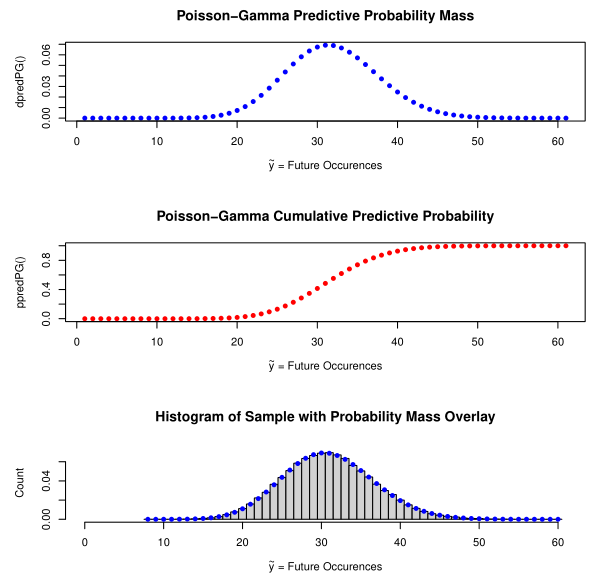
\includegraphics[width=0.95\textwidth]{./Graphics/DistributionPlots/PoissonGamma}
  \caption{Poisson-Gamma Predictive Distribution}
  \label{fig:PGdist}
\end{figure}

\vspace{2cm}




%%%%%%%%%%%%%%%%%%%%%%%%%%%%%%
%%%%%%%%%%%%%%%%%%%%%%%%%%%%%%

\clearpage

  \subsection{Normal Observation with Normal-Inverse Gamma Prior [5]}

    \subsubsection{One Sample Normal-Inverse Gamma}
      \paragraph{Derivation (Normal-Inverse Gamma, 1-sample)}

\noindent Let $\left\{Y_1,...,Y_N|\theta,\sigma^2\right\}\overset{i.i.d.}{\sim}\text{Normal}\left(\theta,\sigma^2\right)$ (assuming $Y_1,...,Y_N$ are exchangeable).  Then the joint sampling density is

        \begin{flalign*}
          p\left(y_1,...,y_N|\theta,\sigma^2\right)
          &= \prod_{i=1}^N p\left(y_i|\theta,\sigma^2\right)\\
          &\\
          &= \prod_{i=1}^N \dfrac{1}{\sqrt{2\pi\sigma^2}}e^{-\frac{1}{2}\left(\frac{y_i - \theta}{\sigma}\right)^2}\\
          &\\
          &= \left(2\pi\sigma^2\right)^{-\sfrac{N}{2}}e^{-\frac{1}{2}\sum_{i=1}^N\left(\frac{y_i - \theta}{\sigma}\right)^2}, -\infty < \theta < \infty, \sigma^2 > 0\\
        \end{flalign*}

\noindent Following Hoff [5] (p. 74-75), for joint inference on both $\theta$ and $\sigma$, we assign priors

        \begin{flalign*}
          \frac{1}{\sigma^2} &\sim \text{Gamma}\left(\sfrac{\nu_0}{2},\sfrac{\nu_0\sigma_0^2}{2}\right), \nu_0 > 0\\
          &\\
          \theta|\sigma^2 &\sim \text{Normal}\left(\mu_0,\sfrac{\sigma^2}{\kappa_0}\right), -\infty < \mu_0 < \infty,  \kappa_0 > 0\\
        \end{flalign*}

\noindent Hoff [5] suggests $\sigma_0^2$ and $\nu_0$ can be interpreted heuristically as sample variance and sample size, respectively, of prior observations, and that  $\mu_0$ and $\kappa_0$ can be thought of as the sample mean and sample size of prior observations.\\

\noindent From this we derive joint posterior distribution

        \begin{flalign*}
          \left\{\theta|y_1,...,y_N,\sigma^2\right\} &\sim \text{Normal}\left(\mu_N,\sfrac{\sigma^2}{\kappa_N}\right)\\
          &\\
          \left\{\sigma^2|y_1,...,y_N\right\} &\sim \text{Inverse Gamma}\left(\sfrac{\nu_N}{2},\sfrac{\sigma^2_N\nu_N}{2}\right).
        \end{flalign*}

\noindent where

        \begin{flalign*}
          \kappa_N &= \kappa_0 + N\\
          &\\
          \mu_N &= \frac{\kappa_0\mu_0+N\bar{y}}{\kappa_N}\\
          &\\
          \nu_N &= \nu_0 + N\\
          &\\
          \sigma_N^2 &= \frac{1}{\nu_N}\left[\nu_0\sigma_0^2 + (N-1)s^2 + \frac{\kappa_0 N}{\kappa_N}\left(\bar{y}-\mu_0\right)^2\right].\\
        \end{flalign*}

\noindent Here $\bar{y} = \frac{1}{N}\sum_{i=1}^N y_i$ is the sample mean and $s^2 = \frac{1}{N-1}\sum_{i=1}^N\left(y_i - \bar{y}\right)^2$ is the sample variance.\\

\noindent From the joint posterior distribution we generate samples by means of the Monte Carlo method (Hoff, p. 77) [5]:

        \begin{flalign*}
          \begin{matrix}
            \sigma^{2(1)}\sim \text{Inverse Gamma}\left(\nu_N/2,\sigma^2_N\nu_N/2\right), & \theta^{(1)}\sim \text{Normal}\left(\mu_N,\sigma^{2(1)}/\kappa_N\right) \\
            \vdots  & \vdots  \\
            \sigma^{2(S)}\sim \text{Inverse Gamma}\left(\nu_N/2,\sigma^2_N\nu_N/2\right), & \theta^{(S)}\sim \text{Normal}\left(\mu_N,\sigma^{2(S)}/\kappa_N\right) \\
          \end{matrix}
        \end{flalign*}

\noindent For prediction of future $\tilde{y}|y_1,...,y_N,\theta,\sigma^2$, generate $\tilde{y}_i \sim \text{Normal}\left(\theta^{(i)},\sigma^{2(i)}\right), i\in\{1,...,S\}$.\\

\noindent For prediction without the influence of any previous knowledge (Hoff p. 79 [5]), we can employ Jeffreys prior $\pi\left(\theta,\sigma^2\right) = 1/\sigma^2$.  This leads to the same conditional distribution for $\theta$ but a Gamma$\left(\frac{N-1}{2},\frac{1}{2}\sum\left(y_i - \bar{y}\right)^2\right)$ distribution for $1/\sigma^2$.  This joint posterior can be integrated to show that
        $$\dfrac{\theta-\bar{y}}{s/\sqrt{N}}|y_1,...,y_N\sim t_{N-1}.$$
\noindent The resulting predictive distribution for $\tilde{y}$ is a t-distribution with location $\bar{y}$ and scale $s\sqrt{1+1/N}$ and $N-1$ degrees of freedom (Gelman et. al. p. 66 [4]).


      \paragraph{R Implementation (Normal-Inverse Gamma, 1-sample)}\label{sec:NormIG1imp}
      R functions \texttt{dpredNormIG1()}, \texttt{ppredNormIG1()}, and \texttt{rpredNormIG1()} have been created for the Normal-Inverse Gamma distribution for density, cumulative probability, and predictive sampling, respectively (see appendix).  These functions all include options for implementation with or without previous knowledge as desired.  If Jeffreys prior is used, the functions simply implement R's Student's t-distribution functions \texttt{rt()}, \texttt{dt()}, and \texttt{pt()}, applying the location and scale parameters as described above.  For predictions using previous knowledge, the functions work as follows:  For the predictive sampler \texttt{rpredNormIG1()}, the Monte Carlo method described above is directly employed.  The predictive density and cumulative predictive density functions (\texttt{dpredNormIG1()} and \texttt{ppredNormID1()}, respectively) depend on the predictive sample. That is, the distributions generated by these two functions are approximated from a sample returned by \texttt{rpredNormIG1()}.\\

\noindent\texttt{ppredNormIG1()} utilizes the empirical cumulative density function \texttt{ecdf()} from R's stats package.  \texttt{dpredNormIG1()} utilizes a Kernel Density Estimation (KDE) method and R's built-in \texttt{density()} function.  The KDE is computed by definition, using a Normal kernel:

      $$\hat{f}_K(x) = \frac{1}{N}\sum_{i=1}^N\frac{1}{h}K\left(\frac{x-X_i}{h}\right),$$

\noindent where

      \begin{flalign*}
        X_i & \text{ is the predictive sample generated using }\texttt{rpredNormIG1()}\\
        &\\
        K & \text{ is Normal}(0,1)\\
        &\\
        h & \text{ is the bandwidth from R's }\texttt{density()}\text{ function (that is, } \texttt{h = density(X}_\texttt{i}\texttt{)\$bw)}\\
      \end{flalign*}

Calls to these functions appear as follows:

\begin{center}
  \texttt{\hyperref[sec:dpredNormIG1]{dpredNormIG1(ypred,y,mu0,k0,sig20,nu0,S,Jeffreys)}}\\
  \texttt{\hyperref[sec:ppredNormIG1]{ppredNormIG1(ypred,y,mu0,k0,sig20,nu0,S,Jeffreys)}}\\
  \texttt{\hyperref[sec:rpredNormIG1]{rpredNormIG1(S,y,mu0,k0,sig20,nu0,Jeffreys)}}\\
\end{center}

\noindent where

\begin{flalign*}
  \texttt{ypred} &= \tilde{y} \text{, value(s) for which prediction is desired}\\
  \texttt{y} &= \mathbf{y} \text{, the observed data}\\
  \texttt{mu0} &= \mu_0 \text{, prior parameter for }\theta\text{, representing the mean of prior observations}\\
  \texttt{k0} &= \kappa_0 \text{, prior parameter for }\theta\text{, representing the sample size of prior observations}\\
  \texttt{sig20} &= \sigma^2_0 \text{, prior parameter for }\sigma^2\text{, representing the variance of prior observations}\\
  \texttt{nu0} &= \nu_0 \text{, prior parameter for }\sigma^2\text{, representing the sample size of prior observations}\\
  \texttt{S} &= S \text{, the desired number of predictions to be generated}\\
  \texttt{Jeffreys} &= \text{ flag (defaulting to }\texttt{FALSE}\text{), controlling the decision to use Jeffrey's prior}
\end{flalign*}


\noindent These functions are exercised in the following example.\\


      \paragraph{Example (Normal-Inverse Gamma, 1-sample) [5]}

        \textit{Example (Hoff p. 72ff [5], using data from Grogan and Wirth (1981)):  Midge wing length}\\

        Grogan and Wirth (1981) provide 9 measurements of midge wing length, in millimeters:  $y = \{1.64, 1.7, 1.72, 1.74, 1.82, 1.82, 1.82, 1.90, 2.08\}$. Previous studies suggest values $\mu_0 = 1.9$ and $\sigma_0^2 = 0.01$.  We choose $\kappa_0 = \nu_0 = 1$ ``...so that our prior distributions are only weakly centered around these estimates from other populations" (Hoff p. 76 [5]). We compute

        \begin{flalign*}
          \bar{y} &= 1.804\\
          &\\
          \text{var}(y) &= 0.0169\\
          &\\
          \kappa_N &= 1 + 9 = 10\\
          &\\
          \mu_N &= \frac{1 \cdot 1.9 + 9 \cdot 1.804}{10} = 1.814\\
          &\\
          \nu_N &= 1 + 9 = 10\\
          &\\
          \sigma_N^2 &= \frac{1}{10}\left[1 \cdot 0.01 + (9-1) \cdot 0.0169 + \frac{1 \cdot 9}{10}\left(1.804 - 1\right)^2\right] = 0.0153\\
        \end{flalign*}

\noindent Thus $\sfrac{\nu_N}{2} = 5$ and $\sfrac{\nu_N\sigma_N^2}{2} = 0.7662$ and we have posteriors

        \begin{flalign*}
          \left\{\theta|y_1,...,y_N,\sigma^2\right\} &\sim \text{Normal}\left(1.814,\sfrac{\sigma^2}{10}\right)\\
          &\\
          \left\{\sigma^2|y_1,...,y_N\right\} &\sim \text{Inverse Gamma}(5,0.7662)\\
        \end{flalign*}

\noindent In Figure \ref{fig:NormIG1dist} below, results from the use of prior knowledge about the population mean are compared to results from using Jeffrey's (non-informative) prior.  Note the robustness of the predictive distribution to the prior choice of mean.  In the top plot showing the estimated density of a predictive sample returned by \texttt{rpredNormIG1()} we see that even prior mean values completely below and completely above the observed data yield distributions with substantial overlap.\\

\begin{figure}[ht]
  \centering
  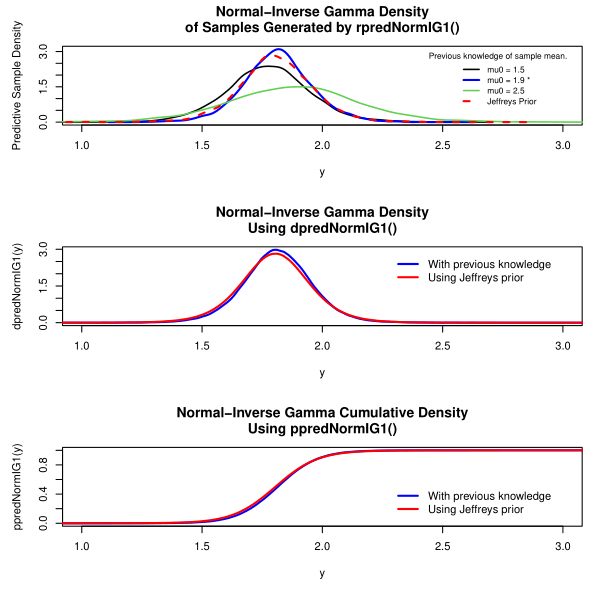
\includegraphics[width=0.95\textwidth]{./Graphics/DistributionPlots/NormIG1}
  \caption{Normal-Inverse Gamma (One-Sample) Predictive Distribution}
  \label{fig:NormIG1dist}
\end{figure}

\vspace{2cm}


\clearpage

    \subsubsection{Two-sample Normal-Inverse Gamma}
      \paragraph{Derivation (Normal-Inverse Gamma, 2-Sample)}

        For a Bayesian analysis comparing two groups $Y_{1,1},...,Y_{N_1,1}$ and $Y_{1,2},...,Y_{N_2,2}$ (assuming each group is exchangeable) we use the following sampling model (Hoff p. 127 [5]):

        \begin{flalign*}
          Y_{i,1} &= \mu + \delta + \epsilon_{i,1}\\
          Y_{i,2} &= \mu - \delta + \epsilon_{i,2}\\
          \left\{\epsilon_{i,j}\right\} &\sim\text{i.i.d. Normal}\left(0,\sigma^2\right), \sigma^2 > 0.
        \end{flalign*}

\noindent Letting $\theta_1 = \mu + \delta$ and $\theta_2 = \mu - \delta$ we see that $\delta = \left(\theta_1 - \theta_2\right)/2$ is half the population difference in means, and $\mu = \left(\theta_1 + \theta_2\right)/2$ is the pooled average.  We will assume conjugate prior distributions

        \begin{flalign*}
          \pi\left(\mu,\delta,\sigma^2\right) &= \pi(\mu) \times \pi(\delta) \times \pi\left(\sigma^2\right)\\
          \mu &\sim \text{Normal}\left(\mu_0,\gamma^2_0\right), -\infty < \mu_0 < \infty,  \gamma^2_0>0\\
          \delta &\sim \text{Normal}\left(\delta_0,\tau^2_0\right), -\infty < \delta_0 < \infty,  \tau^2_0>0\\
          \sigma^2 &\sim \text{Inverse Gamma}\left(\nu_0/2,\nu_0\sigma^2_0/2\right),\nu_0>0.
        \end{flalign*}

\noindent Here $\nu_0$ as before represents the prior sample size.   The full conditional distributions follow:\\

        \indent $\left\{\mu|\mathbf{y}_1,\mathbf{y}_2,\delta,\sigma^2\right\} \sim \text{Normal}\left(\mu_N,\gamma^2_N\right)$, where

        \begin{flalign*}
          \mu_N &= \gamma^2_N \times \left[\dfrac{\mu_0}{\gamma^2_0} + \dfrac{\sum_{i=1}^{N_1}\left(y_{i,1}-\delta\right) + \sum_{i=1}^{N_2}\left(y_{i,2}+\delta\right)}{\sigma^2}\right]\\
          &\\
          \gamma^2_N &=\left[\dfrac{1}{\gamma^2_0} + \dfrac{\left(N_1 + N_2\right)}{\sigma^2}\right]^{-1}
        \end{flalign*}

        \indent $\left\{\delta|\mathbf{y}_1,\mathbf{y}_2,\mu,\sigma^2\right\} \sim \text{Normal}\left(\delta_N,\tau^2_N\right)$, where

        \begin{flalign*}
          \delta_N &= \tau^2_N \times \left[\dfrac{\delta_0}{\tau^2_0} + \dfrac{\sum_{i=1}^{N_1}\left(y_{i,1}-\mu\right) - \sum_{i=1}^{N_2}\left(y_{i,2}-\mu\right)}{\sigma^2}\right]\\
          &\\
          \tau^2_N &=\left[\dfrac{1}{\tau^2_0} + \dfrac{\left(N_1 + N_2\right)}{\sigma^2}\right]^{-1}
        \end{flalign*}

        \indent $\left\{\sigma^2|\mathbf{y}_1,\mathbf{y}_2,\mu,\delta\right\} \sim \text{Inverse Gamma}\left(\frac{\nu_N}{2},\frac{\nu_N\sigma^2_N}{2}\right)$, where

        \begin{flalign*}
          \nu_N &= \nu_0 + N_1 + N_2\\
          \\
          \nu_N\sigma^2_N &= \nu_0\sigma^2_0 + \sum_{i=1}^{N_1}\left(y_{i,1} - [\mu + \delta]\right)^2 + \sum_{i=1}^{N_2}\left(y_{i,2} - [\mu - \delta]\right)^2\\
        \end{flalign*}



      \paragraph{R Implementation (Normal-Inverse Gamma, 2-sample)}\label{sec:NormIG2imp}

      The predictive sample generator R function \texttt{rpredNormIG2()} implements a Gibbs sampler to approximate the posterior distribution $p\left(\mu,\delta,\sigma^2|\mathbf{y}_1,\mathbf{y}_2\right)$, from which to generate predictions for the two populations as follows:
      \begin{enumerate}
        \item Set initial values $\mu = \frac{\theta_1 + \theta_2}{2}$ and $\delta = \frac{\theta_1 - \theta_2}{2}$
        \item Generate a single $\sigma^2|\mathbf{y_1},\mathbf{y_2},\mu,\delta$
        \item Generate a single $\mu|\mathbf{y_1},\mathbf{y_2},\delta,\sigma^2$
        \item Generate a single $\delta|\mathbf{y_1},\mathbf{y_2},\mu,\sigma^2$
        \item Predict $\tilde{y}_1\sim \text{Normal}\left(\mu+\delta,\sigma^2\right)$ and $\tilde{y}_2\sim \text{Normal}\left(\mu-\delta,\sigma^2\right)$
      \end{enumerate}

\noindent The user provides the two samples $\mathbf{y_1}$ and $\mathbf{y_2}$ along with values for $\mu_0, \sigma^2_0, \delta_0, \tau^2_0, \nu_0$, and desired predictive sample size $S$.  The function returns $S$ \sout{predictions for} samples from the predictive distribution for each of the two populations along with the vectors of generated values for $\mu$, $\delta$, and $\sigma^2$.  Calls to this functions appear as follows:


\begin{center}
  \texttt{\hyperref[sec:rpredNormIG2]{rpredNormIG2(S,y1,y2,mu0,g20,d0,t20,nu0,s20)}}\\
\end{center}

\noindent where

\begin{flalign*}
  \texttt{S} &= S \text{, the desired predictive sample size}\\
  \texttt{y1, y2} &= \mathbf{y_1, y_2} \text{, the two sets of observed data}\\
  \texttt{mu0,g20} &= \mu_0,\gamma^2_0 \text{, prior mean and variance for }\mu\\
  \texttt{d0,t20} &= \delta_0,\tau^2_0 \text{, prior mean and variance for }\delta\\
  \texttt{nu0,s20} &= \nu_0,\sigma^2_0 \text{, prior parameters for the variance of the Normal data error terms}\\
\end{flalign*}

      \paragraph{Example (Normal-Inverse Gamma, 2-Sample)}
\vspace{1cm}
      Hoff [5] (p. 128-129) provides the following example, which we reproduce here.  (\textit{Analysis of math score data})\\

      Math score data for two public high schools in the United States (we'll call them School 1 and School 2) were based on results of a national exam, standardized to produce a nationwide mean of 50 and a standard deviation of 10.  The data consisted of 31 individual scores for School 1 and 28 for School 2. Figure \ref{fig:NormIG2_SchoolData} gives a visual summary of the two data sets.\\

\begin{figure}[ht]
  \centering
  \textbf{Observed Math Score Data for Two Schools}
  \captionsetup{width=0.6\textwidth}
  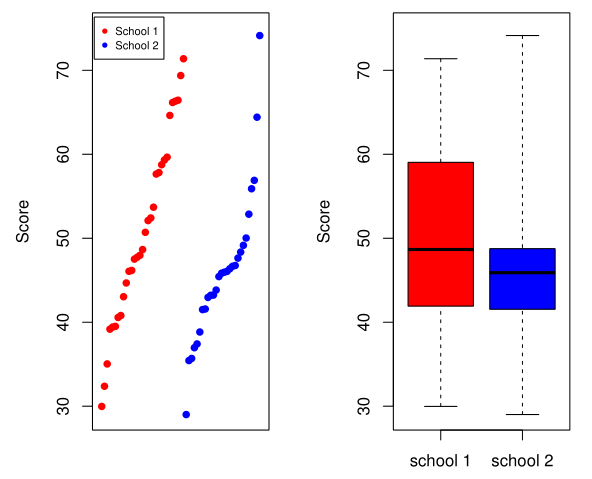
\includegraphics[width=0.8\textwidth]{./Graphics/ExamplePlots/NormIG2_SchoolData}
  \caption{Left-hand plot:  School 1 and School 2 math scores, each arranged by rank, least to greatest.  Right-hand plot:  A box plot of the same data.}
  \label{fig:NormIG2_SchoolData}
\end{figure}


\noindent The mean scores of the two samples are $\bar{y}_1 = 50.81$ and $\bar{y}_2 = 46.15$ for School 1 and School 2, and the standard deviations were $11.3$ and $9.1$, respectively.  A standard t-test yields a $p$-value of $p = 0.087$, in response to which we would fail (at the usual 5\% significance level) to reject the hypothesis that the population means $\theta_1$ and $\theta_2$ are equal. Hoff [5] points out that it is easy to imagine that re-sampling might result in a few more low scores from School 1 and a few more high scores from School 2--enough perhaps to result in a $p$-value below $0.05$ and the opposite conclusion. Why not employ a Bayesian analysis that allows information to be shared across the groups and relies on prior knowledge of the similarities of the two groups?\\

\noindent We're interested in predicting a future math score by a student from each school.  Unless the two schools were known in advance to be extremely exceptional, reasonable prior parameters can be based on this information.  For the prior distributions of $\mu$ and $\sigma^2$, we'll take $\mu_0 = 50$ and $\sigma^2_0 = 10^2 = 100$, although this latter value is likely to be an overestimate of the within-school sampling variability.  We'll make these prior distributions somewhat diffuse, with $\gamma^2_0 = 25^2 = 625$ and $\nu_0 = 1$.  For the prior distribution on $\delta$, choosing $\delta_0 = 0$ represents the prior opinion that $\theta_1 > \theta_2$ and $\theta_2 > \theta_1$ are equally probable.  Finally, since the scores are bounded between 0 and 100, half the difference between $\theta_1$ and $\theta_2$ must be less than 50 in absolute value, so a value of $\tau^2_0 = 25^2 = 625$ seems reasonably diffuse.\\\\

\noindent The results of a call to \texttt{rpredNormIG2()} with the above input values for $\mathbf{y}_1,\mathbf{y}_2,\mu_0,\sigma^2_0,\delta_0,\tau^2_0$, and $N$ are summarized in Figure \ref{fig:NormIG2_DvP}.\\

\begin{figure}[ht]
  \centering
  \captionsetup{width=0.6\textwidth}
  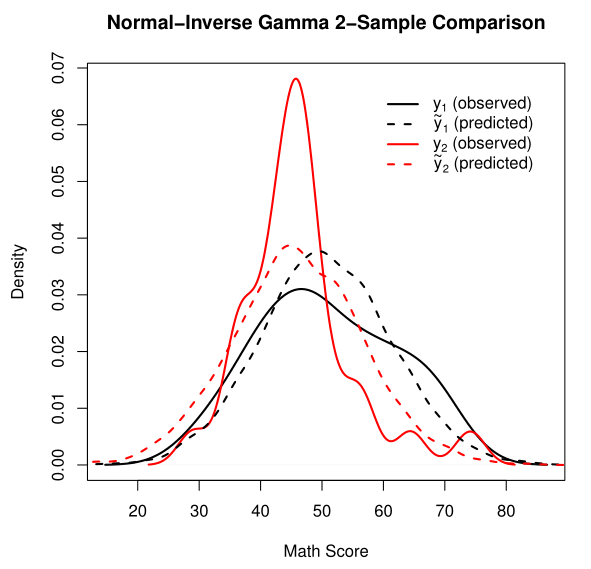
\includegraphics[width=0.8\textwidth]{./Graphics/ExamplePlots/NormIG2_Data_v_Prediction}
  \caption{2-Sample Comparison.  The solid curves show estimated densities based on the observed data.  The dashed curves show the estimated sampling densities of the predictive distributions.}
  \label{fig:NormIG2_DvP}
\end{figure}


\noindent Note that the shared variance but different means from group to group results in predictive densities with very similar shape, but offset from each other in location.  The raw data suggests that it might be useful to explore a model that allows the variances to differ as well.\\

    \subsubsection{$k$-sample Normal-Inverse Gamma:  Comparing multiple groups}

    For two-level data consisting of groups and units within groups, denote data $\mathbf{Y}_1,...,\mathbf{Y_k}$ where $\mathbf{Y}_j = \{Y_{1,j},...,Y_{N_j,j}\}, j=1,...,k$. Here we stipulate exchangeability of $Y_{1,j},...,Y_{N_j,j}$, and thus we can model the data within group $j$ as conditionally i.i.d. given some parameter $\phi_j$.  We also assume that $\phi_1,...,\phi_k$ are exchangeable and thus conditionally i.i.d. given a parameter $\psi$, which has prior distribution $\pi(\psi)$.\\

\noindent We have the hierarchical Normal model (Hoff p. 132 [5]):
    $$\phi_j = \left\{\theta_j,\sigma^2\right\}, p\left(y|\phi_j\right) = \text{Normal}\left(\theta_j,\sigma^2\right), \sigma^2 > 0 \text{ (within-group model)}$$
    $$\psi = \left\{\mu,\tau^2\right\}, p\left(\theta_j|\psi\right) = \text{Normal}\left(\mu,\tau^2\right), \tau^2 > 0 \text{ (between-groups model)}$$

\noindent We use standard semiconjugate Normal and Inverse Gamma prior distributions for the fixed but unknown parameters in the model:
    \begin{flalign*}
      \sigma^2 &\sim \text{Inverse Gamma}\left(\frac{\nu_0}{2},\frac{\nu_0\sigma^2_0}{2}\right), \nu_0 > 0\\
      &\\
      \tau^2 &\sim \text{Inverse Gamma}\left(\frac{\eta_0}{2},\frac{\eta_0\tau^2_0}{2}\right), \eta_0 > 0\\
      &\\
      \mu &\sim \text{Normal}\left(\mu_0,\gamma^2_0\right), -\infty < \mu_0 < \infty, \gamma^2_0 > 0\\
    \end{flalign*}

      \paragraph{Derivation}
      As with the two-sample problem, joint posterior inferences for the unknown parameters can be made by constructing a Gibbs sampler to approximate the posterior distribution $p\left(\theta_1,...,\theta_k,\mu,\tau^2,\sigma^2|\mathbf{y_1,...,y_k}\right)$.  For this we need the full conditional distribution of each parameter (Hoff pp. 134-135 [5]):
      $$\left\{\mu|\theta_1,...,\theta_k,\tau^2\right\} \sim \text{Normal}\left(\dfrac{\frac{k\bar{\theta}}{\tau^2} + \frac{\mu_0}{\gamma^2_0}}{\frac{k}{\tau^2} + \frac{1}{\gamma^2_0}},\dfrac{1}{\frac{k}{\tau^2}+\frac{1}{\gamma^2_0}}\right)$$
      $$\left\{\tau^2|\theta_1,...,\theta_k,\mu\right\} \sim \text{Inverse Gamma}\left(\dfrac{\eta_0 + k}{2},\dfrac{\eta_0\tau^2_0 + \sum\left(\theta_j-\mu\right)^2}{2}\right)$$

      $$\left\{\theta_j|y_{1,j},...,y_{N,j},\sigma^2\right\} \sim \text{Normal}\left(\dfrac{\frac{N_j\bar{y}_j}{\sigma^2} + \frac{1}{\tau^2}}{\frac{N_j}{\sigma^2}+\frac{1}{\tau^2}},\dfrac{1}{\frac{N_j}{\sigma^2}+\frac{1}{\tau^2}}\right)$$

      $$\left\{\sigma^2|\theta_1,...,\theta_k,\mathbf{y_1,...,y_k}\right\} \sim \text{Inverse Gamma}\left(\dfrac{1}{2}\left[\nu_0 + \sum_{j=1}^k N_j\right],\dfrac{1}{2}\left[\nu_0\sigma^2_0 + \sum_{j=1}^k\sum_{i=1}^{N_j}\left(y_{i,j}-\theta_j\right)^2\right]\right).$$

\noindent Here $\bar{\theta} = \frac{1}{k}\sum_{j=1}^k \theta_j$.  Note that $\sum\sum\left(y_{i,j}-\theta_j\right)^2$ is the sum of squared residuals across all groups, conditional on the within-group means, and so the conditional distribution concentrates probability around a pooled-sample estimate of the variance.\\

\noindent Finally, a prediction for the $j^{\text{th}}$ group is given by
$$\tilde{y}_j \sim \text{Normal}(\theta_j, \sigma^2).$$

      \paragraph{R Implementation (Normal-Inverse Gamma, k-samples)}\label{sec:NormIGkimp}

      The R function \texttt{rpredNormIGk()} implements a Gibbs sampler for posterior approximation of each unknown quantity by sampling from its full conditional distribution.  From these posteriors, predictions are generated, as follows:

      \begin{enumerate}
        \item Set prior parameter values:
          \begin{flalign*}
            \nu_0,\sigma^2_0 \text{ for } \pi\left(\sigma^2\right)\\
            \eta_0,\tau^2_0 \text{ for } \pi\left(\tau^2\right)\\
            \mu_0,\gamma^2_0 \text{ for } \pi\left(\mu\right).
          \end{flalign*}
        \item Set initial states for the unknown parameters:
          \begin{flalign*}
            \theta_1^{(1)} &= \mathbf{\bar{y}_1},...,\theta_k^{(1)} = \mathbf{\bar{y}_k}\\
            \mu^{(1)} &= \text{mean}\left(\theta_1^{(1)},...,\theta_k^{(1)}\right)\\
            \tau^{2(1)} &= \text{var}\left(\theta_1^{(1)},...,\theta_k^{(1)}\right)\\
            \sigma^{2(1)} &= \text{mean}\left(\text{var}\left(\mathbf{y}_1\right),...,\text{var}\left(\mathbf{y}_k\right)\right)
          \end{flalign*}
        \item For $s\in\{1,...,S\}$, sample
          \begin{enumerate}
            \item $\mu^{(s+1)} \sim p\left(\mu|\theta_1^{(s)},...,\theta_k^{(s)},\tau^{2(s)}\right)$
            \item $\tau^{2(s+1)} \sim p\left(\tau^2|\theta_1^{(s)},...,\theta_k^{(s)},\mu^{(s+1)}\right)$
            \item $\sigma^{2(s+1)} \sim p\left(\sigma^2|\theta_1^{(s)},...,\theta_k^{(s)},\mathbf{y}_1,...,\mathbf{y}_k\right)$
            \item $\theta_j^{(s+1)} \sim p\left(\theta_j|\mu^{(s+1)},\tau^{2(s+1)},\sigma^{2(s+1)},\mathbf{y}_j\right)$ for $j \in \{1,...,k\}$
          \end{enumerate}
        \item For $s\in\{1,...,S\}$, generate prediction $\tilde{y}_j^{(s)} \sim \text{Normal}\left(\theta_j^{(s)},\sigma^{2(s)}\right)$ for $j \in \{1,...,k\}$
      \end{enumerate}

\noindent Calls to this functions appear as follows:


\begin{center}
  \texttt{\hyperref[sec:rpredNormIGk]{rpredNormIGk(S,Y,nu0,s20,eta0,t20,mu0,g20)}}\\
\end{center}

\noindent where

\begin{flalign*}
  \texttt{S} &=S \text{, the desired predictive sample size. The sampler returns } S \text{ realizations}\\
  &\text{from the predictive distribution, each having } k \text{ elements, one corresponding to}\\
  &\text{each data group } \mathbf{Y}_1,...,\mathbf{Y_k} \text{. That is, } \mathbf{\tilde{Y}_j} = \tilde{Y}_{1,j},...,\tilde{Y}_{s,j} \text{, for } j \in \{1,...,k\}, s\in\{1,...S\}.\\
  \texttt{Y} &= \text{ the } k \text{ sets of observed data (one column of data and one column of}\\ &\text{group indices)}
\end{flalign*}
\begin{flalign*}
  \texttt{nu0} &= \nu_0 \text{, prior parameter for } \sigma^2 \text{ representing prior sample size}\\
  \texttt{s20} &= \sigma^2_0 \text{, prior parameter for } \sigma^2 \text{ representing within-sample variance}\\
  \texttt{eta0} &= \eta_0 \text{, prior parameter for } \tau^2 \text{ representing prior sample size}\\
  \texttt{t20} &= \tau^2_0 \text{, prior parameter for } \tau^2 \text{ representing between-sample variance}\\
  \texttt{mu0} &= \mu_0 \text{, prior parameter for } \mu \text{ representing the mean of the pooled average}\\ &\text{from prior knowledge}\\
  \texttt{g20} &= \gamma^2_0 \text{, prior parameter for } \mu \text{ representing the variance of the pooled average}\\ &\text{from prior knowledge}
\end{flalign*}



      \paragraph{Example}
      Returning to the math scores example, data for 10th-grade students from 100 large urban schools (each having 10th-grade enrollment of at least 400) is summarized in Figure \ref{fig:NormIGk_All100}. %Each school's results are represented by a vertical segment, with points plotted at the individual students' math scores. The horizontal line is drawn at the grand mean of the individual school means.

\begin{figure}[ht]
  \centering
  \captionsetup{width=0.6\textwidth}
  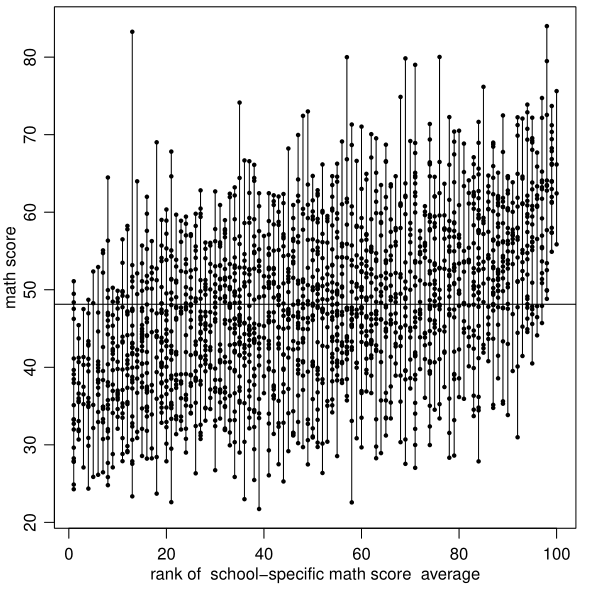
\includegraphics[width=0.8\textwidth]{./Graphics/ExamplePlots/NormIGk_MathScoreData}
  \caption{Math Score Data for 100 Schools.  Each school's results are represented by a vertical segment, with points plotted at the individual students' math scores. The horizontal line is drawn at the grand mean of the individual school means.}
  \label{fig:NormIGk_All100}
\end{figure}


\clearpage

\noindent For prediction, we'll use the following prior values (Hoff p. 137 [5]):

      \begin{flalign*}
        \sigma^2_0&:  100 \text{ (within-school variance)}\\
        \nu_0&:  1 \text{ (prior sample size)}\\
        \tau^2_0&:  100 \text{ (between-school variance)}\\
        \eta_0&:  1 \text{ (prior sample size)}\\
        \mu_0&:  50 \text{ (prior mean of school means)}\\
        \gamma^2_0&:  25 \text{ (prior variance of school means)}
      \end{flalign*}

\noindent In the example below the observed test score data from three individual schools are compared with their predictions.  The schools chosen were numbers 5, 67, and 92 from the study, which had the minimum average math score, maximum average math score, and closest to the overall average math score, respectively.  These values are recorded in the table here:


\begin{center}
  \begin{tabular}{|c|c|c|}
    \hline
    & school & average \\
    \hline
    min average & 5 & 36.58 \\
    \hline
    max average & 67 & 65.02 \\
    \hline
    grand mean & -- & 48.13 \\
    \hline
    closest to overall & 92 & 48.18\\
    \hline
  \end{tabular}
\end{center}

\clearpage

\noindent Figure \ref{fig:NormIGk_DvP} shows the estimated density curves of the observed math scores for these three schools and the predictive density of an unobserved student's score from each school.  The densities are represented with solid lines for observed data and dashed lines for predicted quantities.  The predictive densities are ``pulled" toward the overall mean, which is indicated on the plot with the dotted gray vertical line.

\begin{figure}[h]
  \centering
  \captionsetup{width=0.6\textwidth}
  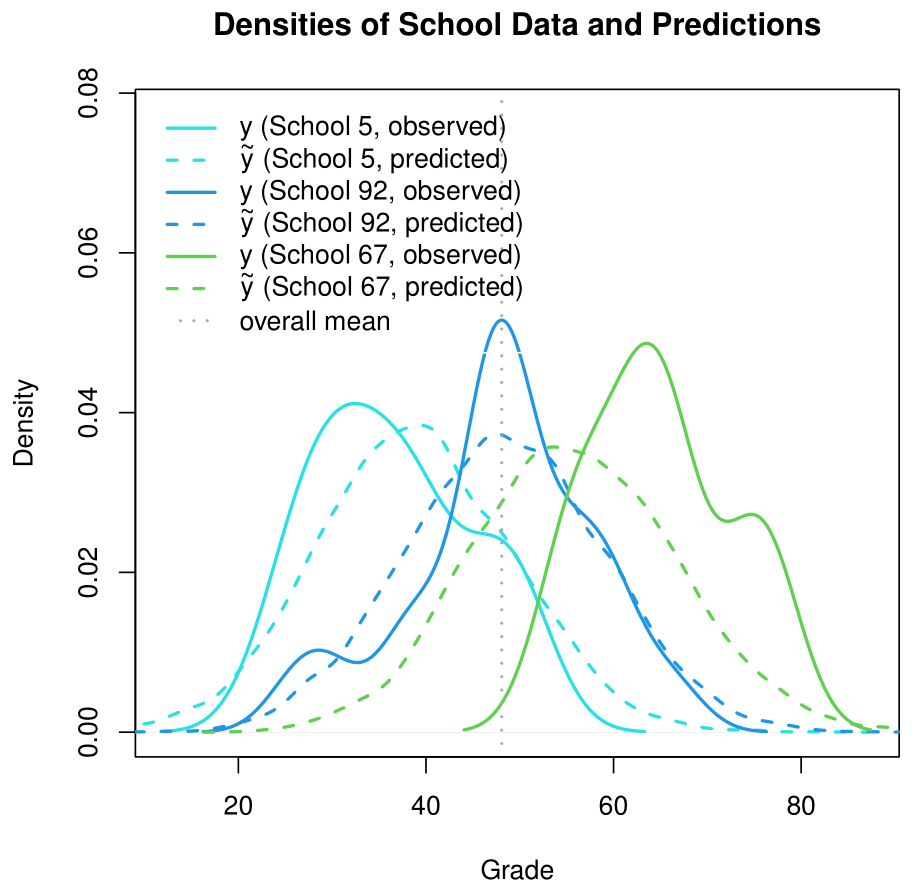
\includegraphics[width=0.8\textwidth]{./Graphics/ExamplePlots/NormIGk_Data_v_Prediction}
  \caption{$k$-Sample Comparison. The solid curves show estimated densities based on the observed data.  The dashed curves show the estimated sampling densities of the predictive distributions.}
  \label{fig:NormIGk_DvP}
\end{figure}



      % \paragraph{Ranking Treatments}

\clearpage


\section{Normal Regression [5]}% with Zellner's $g$-prior}

% \textcolor{red}{intro here}\\
% \textcolor{red}{stipulate variable naming convention here (x is the observed data now).  Modify previous intro to indicate variable convention was for the exponential family set of models}

\noindent Starting with observations $Y_1,...,Y_N$ and explanatory variables $\mathbf{x}_1,...,\mathbf{x}_N$, with $\mathbf{x}_i = \left\{ x_{i,1}, x_{i,2}, ..., x_{i,p} \right\}$ where $Y_i = \boldsymbol\beta^T \mathbf{x}_i + \epsilon_i$ and $\epsilon_1,...,\epsilon_n\overset{\text{i.i.d.}}{\sim} \text{Normal}\left(0,\sigma^2\right)$, we have joint probability density

\begin{flalign}
    p\left(y_1,...y_N|\mathbf{x}_1,...,\mathbf{x}_N,\boldsymbol\beta,\sigma^2\right) &= \prod_{i=1}^N p\left(y_i|\mathbf{x}_i,\boldsymbol\beta,\sigma^2\right) \nonumber\\
    &= \left(2\pi\sigma^2\right)^{-N/2}\text{exp}\left\{-\frac{1}{2\sigma^2}\sum_{i=1}^n\left(y_i - \boldsymbol\beta^T\mathbf{x}_i\right)^2\right\}. \label{regressionJointNorm}
\end{flalign}

\noindent If we let $\mathbf{y}=(y_1,...,y_N)^T$ and let $\mathbf{X}$ be the $n \times p$ matrix whose $i$th row is $\mathbf{x}_i$, then we can express this joint probability in terms of the Multivariate Normal distribution.  The Normal regression model is

$$\{\mathbf{y}|\mathbf{X},\boldsymbol\beta,\sigma^2\} \sim \text{Multivariate Normal}\left(\mathbf{X}\boldsymbol\beta,\sigma^2\mathbf{I}\right),$$

\noindent where $\mathbf{I}$ is the $p \times p$ identity matrix and

\begin{equation*}
    \mathbf{X}\boldsymbol\beta =
    \begin{pmatrix}
        \mathbf{x}_1 \\
        \mathbf{x}_2 \\
        \vdots  \\
        \mathbf{x}_N
    \end{pmatrix}
    \begin{pmatrix}
        \beta_1 \\
        \beta_2 \\
        \vdots \\
        \beta_p
    \end{pmatrix}
    =
    \begin{pmatrix}
        \beta_1 x_{1,1} + \cdots + \beta_p x_{1,p} \\
        \vdots \\
        \beta_1 x_{N,1} + \cdots + \beta_p x_{N,p} \\
    \end{pmatrix}
    =
    \begin{pmatrix}
        E\left[Y_1|\mathbf{\boldsymbol\beta},\mathbf{x}_1\right] \\
        \vdots \\
        E\left[Y_N|\mathbf{\boldsymbol\beta},\mathbf{x}_N\right] \\
    \end{pmatrix}
\end{equation*}

\noindent The density (\ref{regressionJointNorm}) depends on $\boldsymbol\beta$ through the residuals $\left(y_i - \boldsymbol\beta^T\mathbf{x}_i\right)$.  We compute the ordinary least squares estimates

$$\hat{\boldsymbol\beta}_{ols} = \left(\mathbf{X}^T\mathbf{X}\right)^{-1}\mathbf{X}^T\mathbf{y}$$

\noindent and

$$\hat{\sigma}^2_{ols} = \frac{SSR\left(\hat{\boldsymbol\beta}_{ols}\right)}{(N-p)} = \frac{\sum\left(y_i - \hat{\boldsymbol\beta}_{ols}^T x_i\right)^2}{(N-p)}.$$


\noindent Here

\begin{flalign*}
  SSR(\beta) &= \sum_{i=1}^N(y_i-\beta^T x_i)^2\\
              &= \sum_{i=1}^N(\mathbf{y-X}\beta)^T(\mathbf{y-X}\beta)\\
              &= \mathbf{y}^T\mathbf{y}-2\beta^T\mathbf{X}^T\mathbf{y} + \beta^T\mathbf{X}^T\mathbf{X}\beta
\end{flalign*}

\noindent is the sum of squared residuals, which is minimized by $\hat\beta_{ols}$.\\


\subsection{Least Squares Estimation Example}

\noindent Here we reproduce the example provided by Hoff (p. 149ff) [5], which will be used to illustrate Bayesian prediction for a regression model.\\

\noindent\textit{Example:  Oxygen Uptake [5]}

\noindent Twelve healthy men who did not exercise regularly were recruited to take part in a study of the effects of two different exercise regimens on oxygen uptake.  Six of the twelve men were randomly assigned to a 12-week flat-terrain running program, and the remaining six were assigned to a 12-week step aerobics program.  The maximum oxygen uptake of each subject was measured (in liters per minute) while running on an inclined treadmill, both before and after the 12-week program.  Of interest is how a subject's change in maximal oxygen uptake may depend on which program they were assigned to.  However, other factors, such as age, are expected to affect the change in maximal uptake as well.  The results are shown in Figure \ref{fig:OxygenData}:

\begin{figure}[ht]
  \centering
  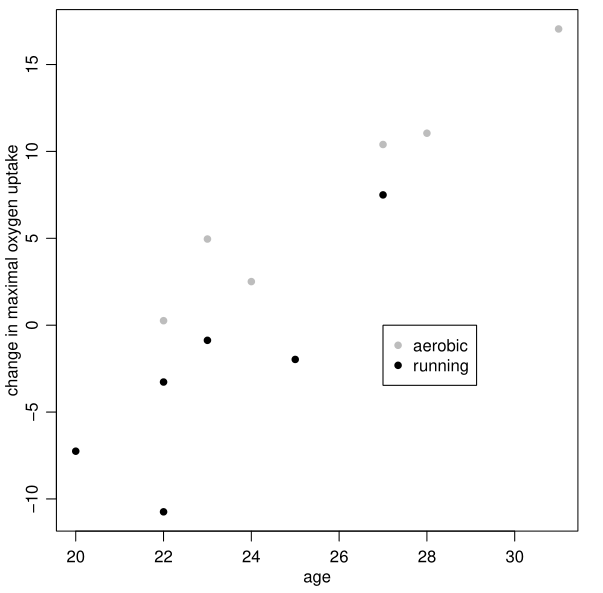
\includegraphics[width=0.8\textwidth]{./Graphics/ExamplePlots/OxygenUptakeData}
  \caption{Oxygen Uptake Data}
  \label{fig:OxygenData}
\end{figure}


\clearpage

\noindent Hoff [5] suggests the following regression model for this data:

    \begin{align}
        Y_i &= \beta_1x_{i,1} + \beta_2x_{i,2} + \beta_3x_{i,3} + \beta_4x_{i,4} + \epsilon_i, \text{ where} \label{example_regression_model}\\
        x_{i,1} &= 1 \text{ for each subject } i \nonumber \\
        x_{i,2} &= 0 \text{ if subject } i \text{ is on the running program, } 1 \text{ if on aerobic} \nonumber \\
        x_{i,3} &= \text{ age of subject } i \nonumber \\
        x_{i,4} &= x_{i,2} \times x_{i,3} \nonumber
    \end{align}

\noindent Under this model the conditional expectations of $Y$ for the two different levels of $x_{i,2}$ are

\begin{flalign*}
    E[Y|\mathbf{x}] &= \beta_1 + \beta_3 \times age \text{ if } x_{i,2} = 0 \text{ (running program), and}\\
    E[Y|\mathbf{x}] &= \left(\beta_1 + \beta_2\right) + \left(\beta_3 + \beta_4\right) \times age \text{ if } x_{i,2} = 1 \text{ (aerobic program) }
\end{flalign*}

\noindent In other words, the model assumes that the relationship is linear in age for both exercise groups, with the difference in intercepts given by $\beta_2$ and the difference in slopes given by $\beta_4$.  If we assumed that $\beta_2 = \beta_4 = 0$, then we would have identical lines for both groups.  If we assumed $\beta_2 \ne 0$ and $\beta_4 =  0$ then we would have a different line for each group but they would be parallel.  Allowing all coefficients to be non-zero gives us two unrelated lines.  Some different possibilities are depicted graphically in Figure \ref{fig:RegModVar}:\\

\begin{figure}[ht]
  \centering
  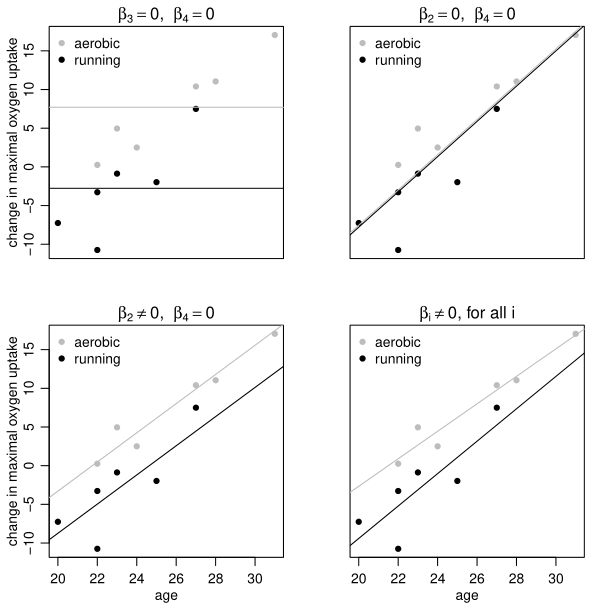
\includegraphics[width=0.8\textwidth]{./Graphics/ExamplePlots/RegressionModelVariations}
  \caption{Regression Model Variations}
  \label{fig:RegModVar}
\end{figure}


\noindent Let's find the least squares regression estimates for the model (\ref{example_regression_model}), and use the results to evaluate the differences between the two exercise groups.  The ages of the 12 subjects, along with their observed changes in maximal oxygen uptake, are

\begin{flalign*}
    \mathbf{x}_3 &= (23,22,22,25,27,20,31,23,27,28,22,24)\\
    \mathbf{y}   &= (-0.87,-10.74,-3.27,-1.97,7.50,-7.25,17.05,4.96,10.40,11.05,0.26,2.51),
\end{flalign*}

\noindent with the first six elements of each vector corresponding to the subjects in the running group and the latter six corresponding to subjects in the aerobics group.  After constructing the $12 \times 4$ matrix $\mathbf{X} = (\mathbf{x}_1\, \mathbf{x}_2\, \mathbf{x}_3\, \mathbf{x}_4)$, the matrices $\mathbf{X}^T\mathbf{X}$ and $\mathbf{X}^T\mathbf{y}$ can be computed, from which we get $\boldsymbol\beta_{ols} = \left(\mathbf{X}^T\mathbf{X}\right)^{-1}\mathbf{X}^T\mathbf{y} = (-51.29,13.11,2.09,-0.32)^T$:\\

\noindent This means that the estimated linear relationship between uptake and age has an intercept and slope of -51.29 and 2.09 for the running group, and -51.29 + 13.11 = -38.18 and 2.09 - 0.32 = 1.77 for the aerobics group.  These two lines are plotted in the fourth panel of Figure XX.  We obtain unbiased estimate $\hat\sigma^2 = SSR(\hat{\boldsymbol\beta}_{ols})/(n-p) = 8.54$, and use this to compute the standard error of the components of $\hat{\boldsymbol\beta}_{ols}$, which are 12.25, 15.76, 0.53, and 0.65, respectively.  Comparing the values of $\hat{\boldsymbol\beta}_{ols}$ to their standard errors suggests that the evidence for differences between the two exercise regimens is not very strong.





\clearpage

  \subsection{Bayesian Estimation for a Regression Model [5]}

  \subsubsection{Derivation (Normal Regression)}

    \paragraph{A semiconjugate prior distribution}\label{normRegSemiconjugatePrior}
    Hoff [5] proposes a semiconjugate prior distribution for $\boldsymbol\beta$ and $\sigma^2$ to be used when there is information available about the parameters.  The sampling density of the data is

    $$p(\mathbf{y}|\mathbf{X},\boldsymbol\beta,\sigma^2) \propto \text{exp}\{-\frac{1}{2\sigma^2}\text{SSR}(\boldsymbol\beta)\} = \text{exp}\{-\frac{1}{2\sigma^2}[\mathbf{y}^T\mathbf{y} - 2\boldsymbol\beta^T\mathbf{X}^T\mathbf{y}+\boldsymbol\beta^T\mathbf{X}^T\mathbf{X}\boldsymbol\beta]\},$$

\noindent and for priors we choose $\boldsymbol\beta \sim \text{Multivariate Normal}(\boldsymbol\beta_0,\Sigma_0)$ and $1/\sigma^2 = \gamma\sim \text{Gamma}(\nu_0/2,\nu_0\sigma^2_0/2)$.  \\

\noindent Thus we have conditional posterior for $\boldsymbol\beta$

    \begin{flalign*}
        p&(\boldsymbol\beta|\mathbf{y,X},\sigma^2)\\
        &\propto p(\mathbf{y}|\mathbf{X},\boldsymbol\beta, \sigma^2) \times p(\boldsymbol\beta)\\
        &\propto \text{exp}\{-\frac{1}{2}(-2\boldsymbol\beta^T\mathbf{X}^T\mathbf{y}/\sigma^2 + \boldsymbol\beta^T\mathbf{X}^T\mathbf{X}\boldsymbol\beta/\sigma^2) - \frac{1}{2}(-2\boldsymbol\beta^T\Sigma_0^{-1}\boldsymbol\beta_0 + \boldsymbol\beta^T\Sigma_0^{-1}\boldsymbol\beta)\}\\
        &=\text{exp}\{\boldsymbol\beta^T(\Sigma_0^{-1}\boldsymbol\beta_0 + \mathbf{X}^T\mathbf{y}/\sigma^2) - \frac{1}{2}\boldsymbol\beta^T(\Sigma_0^{-1} + \mathbf{X}^T\mathbf{X}/\sigma^2)\boldsymbol\beta\}\\
        &\propto \text{MVN}(\mathbf{m,V})
    \end{flalign*}

\noindent where

$$\mathbf{m} = \text{E}[\boldsymbol\beta|\mathbf{y,X},\sigma^2] = \left(\Sigma_0^{-1} + \mathbf{X}^T\mathbf{X}/\sigma^2\right)^{-1}\left(\Sigma_0^{-1}\boldsymbol\beta_0 + \mathbf{X}^T\mathbf{y}/\sigma^2\right)$$

$$\mathbf{V} = \text{Var}[\boldsymbol\beta|\mathbf{y,X},\sigma^2] = \left(\Sigma_0^{-1} + \mathbf{X}^T\mathbf{X}/\sigma^2\right)^{-1},$$

\noindent and conditional posterior for $\gamma$

\begin{flalign*}
    p(\gamma|\mathbf{y,X},\boldsymbol\beta) &\propto p(\gamma)p(\mathbf{y}|\mathbf{X},\boldsymbol\beta,\gamma)\\
        &\propto \left[\gamma^{\nu_0/2-1}\text{exp}(-\gamma \times \nu_0\sigma^2_0/2)\right] \times
                 \left[\gamma^{N/2}\text{exp}(-\gamma \times \text{SSR}(\boldsymbol\beta)/2)\right]\\
        &= \gamma^{(\nu_0+N)/2-1} \text{exp}(-\gamma[\nu_0\sigma^2_0 + \text{SSR}(\boldsymbol\beta)]/2),
\end{flalign*}

\noindent which we recognize as a gamma density, so that

$$\{\sigma^2|\mathbf{y,X},\boldsymbol\beta\} \sim \text{Inverse Gamma}([\nu_0 + N]/2,[\nu_0\sigma^2_0 + \text{SSR}(\boldsymbol\beta)]/2).$$

\vspace{5mm}

\noindent Constructing a Gibbs sampler to approximate the joint posterior distribution $p(\boldsymbol\beta,\sigma^2|\mathbf{y,X})$ is then straightforward:  given current values $\{\boldsymbol\beta^{(s)},\sigma^{2(s)}\}$, new values can be generated by

\begin{enumerate}
    \item updating $\boldsymbol\beta$:
    \begin{enumerate}
        \item compute $\mathbf{m}^{(s)}$ and $\mathbf{V}^{(s)}$
        \item sample $\boldsymbol\beta^{(s+1)} \sim \text{Multivariate Normal}(\mathbf{m^{(s)},V^{(s)}})$
    \end{enumerate}
    \item updating $\sigma^2$:
    \begin{enumerate}
        \item compute SSR$(\boldsymbol\beta^{(s+1)})$
        \item sample $\sigma^{2(s+1)} \sim \text{Inverse Gamma}([\nu_0 + N]/2,[\nu_0\sigma_0^2 + \text{SSR}(\boldsymbol\beta^{(s+1)})]/2)$.
    \end{enumerate}
\end{enumerate}

\noindent To create a sample from the predictive distribution of responses:  for each $s\in\{1,...,S\}$, draw $\epsilon^{(s)} \sim \text{Normal}(0,\sigma^{2(s)})$.  Then compute

$$y^{(s)} = \boldsymbol\beta^{(s)T}\mathbf{X}_p + \epsilon^{(s)}$$

\noindent for the $\mathbf{X}_p$ for which prediction is desired.

    \paragraph{Default and weakly informative prior distributions}

    In situations where prior information is unavailable or difficult to quantify, an alternative ``default" class of prior distributions is given. Here we will employ Zellner's ``$g$-prior" (Zellner, 1986).  We choose $\boldsymbol\beta_0 = \mathbf{0}$ and $\Sigma_0 = k(\mathbf{X}^T\mathbf{X})^{-1}, k = g\sigma^2, g > 0$, which satisfies a desired condition that the regression parameter estimation be invariant to changes in the scale of the regressors.  Note that this prior conditions on the observed $\mathbf{X}$ matrix.With this, $\mathbf{m}=\text{E}[\boldsymbol\beta|\mathbf{y,X},\sigma^2]$ and $\mathbf{V}=\text{Var}[\boldsymbol\beta|\mathbf{y,X},\sigma^2]$ reduce to

\begin{flalign}
    \text{E}[\boldsymbol\beta|\mathbf{y,X},\sigma^2] &= [\mathbf{X^TX}/(g\sigma^2) + \mathbf{X^TX}/\sigma^2]^{-1}\mathbf{X^Ty}/\sigma^2 = \frac{g}{g+1}\sigma^2(\mathbf{X^TX})^{-1}\mathbf{X^Ty}.\label{regression_noninf_expec}\\
    \text{Var}[\boldsymbol\beta|\mathbf{y,X},\sigma^2] &= [\mathbf{X^TX}/(g\sigma^2) + \mathbf{X^TX}/\sigma^2]^{-1} = \frac{g}{g+1}\sigma^2(\mathbf{X^TX})^{-1} \label{regression_noninf_var}
\end{flalign}

\noindent Letting

$$\mathbf{V} = \frac{g}{g+1}\sigma^2(\mathbf{X^TX})^{-1} \text{ and } \mathbf{m} = \frac{g}{g+1}\sigma^2(\mathbf{X^TX})^{-1}\mathbf{X^Ty}$$

\noindent we arrive at posteriors

\begin{flalign}
    \{\sigma^2|\mathbf{y,X}\} &\sim \text{Inverse Gamma}([\nu_0 + n]/2,[\nu_0\sigma^2_0 + \text{SSR}_g]/2) \label{regression_noninf_sig2_post}\\
    \{\boldsymbol\beta|\mathbf{y,X},\sigma^2\} &\sim \text{Multivariate Normal}\left(\frac{g}{g+1}\hat{\boldsymbol\beta}_{ols},\frac{g}{g+1}\sigma^2[\mathbf{X^TX}]^{-1}\right).\label{regression_noninf_beta_post}
\end{flalign}

\noindent Here $\text{SSR}_g = \mathbf{y^Ty - m^TV^{-1}m = y^T(I - }\frac{g}{g+1}\mathbf{X(X^TX)^{-1}X^T)y}$.\\

Simple Monte Carlo approximation can be used to sample from the joint posterior density $p(\sigma^2,\boldsymbol\beta|\mathbf{y,X})$ as follows.  Here $g$ is typically set to the size of the data sample (i.e. $g = N$). Then:

\begin{enumerate}
    \item sample $\sigma^2 \sim \text{Inverse Gamma}([\nu_0 + N]/2,[\nu_0\sigma^2_0 + \text{SSR}_g]/2)$
    \item sample $\boldsymbol\beta \sim \text{Multivariate Normal}\left(\frac{g}{g+1}\hat{\boldsymbol\beta}_{ols},\frac{g}{g+1}\sigma^2[\mathbf{X^TX}]^{-1}\right)$.
\end{enumerate}

\noindent To create a sample from the predictive distribution of responses, draw $\epsilon \sim \text{Normal}(0,\sigma^2)$.  Then for each triplet $(\beta,\sigma^2,\epsilon)$ we have

$$y = \boldsymbol\beta^T\mathbf{X} + \epsilon.$$

  \subsubsection{R Implementation (Normal Regression)}\label{sec:NormRegimp}

The R function \texttt{rpredNormReg()} returns a sample from the predictive distribution $y = X_{pred}\boldsymbol\beta^{(s)} + \epsilon^{(s)}$ for each $s$.  It does this by approximating the joint posterior density $p(\sigma^2,\boldsymbol\beta|\mathbf{y,X})$ using one of the two methods described above and generating $S$ triplets $(\boldsymbol\beta^{(s)}, \sigma^{2(s)},\epsilon^{(s)}), s \in 1,...,S$.  Calls to this functions appear as follows:

\begin{center}
  \texttt{\hyperref[sec:rpredNormReg]{rpredNormReg(S,Xpred,X,y,beta0,Sigma0,nu0,s20,gprior)}}\\
\end{center}

\noindent where

\begin{flalign*}
  \texttt{S} &= S \text{, the number of MCMC realizations (the desired predictive sample size)}\\
  \texttt{Xpred} &= \text{ the vector or matrix of vectors of explanatory variables upon which to base}\\ &\text{prediction }\\
  \texttt{X} &= \mathbf{X} \text{, the design matrix associated with the observed data}\\
  \texttt{y} &= \mathbf{y} \text{, the observed response vector}\\
  \texttt{beta0} &= \beta_0 \text{, location vector for the Multivariate Normal prior distribution of } \mathbf{\beta}\\
  \texttt{Sigma0} &= \Sigma_0 \text{, covariance matrix for the Multivariate Normal prior distribution of } \mathbf{\beta}\\
  \texttt{nu0,s20} &= \nu_0,\sigma^2_0 \text{, prior parameters for the Inverse-Gamma prior distribution of }\sigma^2\\
  \texttt{gprior} &= \text{ a flag controlling the decision to use Zellner's location-invariant g-prior}
\end{flalign*}

\noindent Note:  the function defaults to \texttt{gprior=TRUE}, in which case input values for \texttt{beta0, Sigma0, nu0}, and \texttt{s20} are ignored.  If the user wants to employ Hoff's semi-conjugate prior as defined in section \ref{normRegSemiconjugatePrior} above, all input variables must be specified, with \texttt{gprior = FALSE}.




  \subsubsection{Example (Normal Regression)}

In the example below (Hoff data and code found \href{https://pdhoff.github.io/book/}{https://pdhoff.github.io/book/}) to employ Hoff's semi-conjugate prior we use



\begin{flalign*}
  \boldsymbol\beta_0 &= \hat{\boldsymbol\beta}_{ols} = (-51.29, 13.11, 2.09, -0.32)  \text{ (ordinary least squares estimator of } \boldsymbol\beta \text{)}\\
  \Sigma_0 &= (\mathbf{X}^T\mathbf{X})^{-1}\sigma^2 =
    \begin{pmatrix}
      150.12 & -150.12 & -6.42 & 6.42 \\
      -150.12 & 248.44 & 6.42 & -10.17 \\
      -6.42 & 6.42 & 0.28 & -0.28 \\
      6.42 & -10.17 & -0.28 & 0.42
    \end{pmatrix}
    \text{ (sampling variance of } \hat{\boldsymbol\beta}_{ols}\text{)}\\%\text{WHY TIMES n????}\\
  \nu_0 &= 1 \text{ (prior sample size)}\\
  \sigma^2_0 &= \frac{\sum e_i}{N-p} = 6.21 \text{ (variance of the residuals)}\\
  S &= 5000 \text{, the predictive sample size}
\end{flalign*}


\noindent Inspection of the plot in Figure \ref{fig:RegPriorComp} shows the predicted distributions using Zellner's g-prior shrink toward 0, and have greater variance than those predicted using Hoff's semi-conjugate prior.

\begin{figure}[ht]
  \centering
  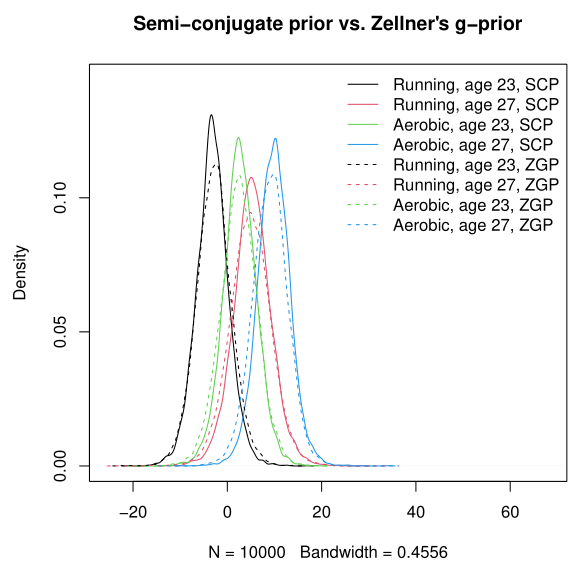
\includegraphics[width=0.8\textwidth]{./Graphics/ExamplePlots/RegressionPriorComparison}
  \caption{Regression Prediction Comparison}
  \label{fig:RegPriorComp}
\end{figure}



\clearpage

\section{Conclusion}

The need to forecast future events arises in a broad array of disciplines: across all the sciences, in politics, in sports, in business, in finance---the list goes on.  Decisions influenced by forecasting often have far-reaching impact.  Scientific research and technological progress can be greatly aided by accurate prediction, for example, for reproducibility, verification of hypotheses, and design cycle efficiency.  Clearly the parties involved in any forward-looking endeavor greatly benefit from a reliable means of prediction.  As such the importance of prediction as an inferential technique is evident, and it behooves the statistician to arrive at the consultation table with a dependable set of predictive tools in hand.\\

\noindent The field of statistics does not lack a body of theory for predictive inference, and statisticians have at their fingertips exponentially expanding computing power.  Bayesian predictive techniques are ripe to be exercised on the mountains of existing data, if the right tools are available.  But the right tools are not generally available---so this thesis begins to respond to that need.  I have developed easy-to-use R functions that implement prediction for several standard classes of problems.  These functions are tested and ready to be used, providing a foundation for a statistical tool set ready to be applied to today's prediction problems.

\clearpage

\section{Appendix - R Functions}

The functions below are part of a package of predictive inference tools.  The package is being developed to be published and made available to the researcher for general use.

  \subsection{Beta-Binomial R Functions}
    \subsubsection{\texttt{dpredBB()}}\label{sec:dpredBB}

    \texttt{\hyperref[sec:BBimp]{dpredBB} <- function(tpred, N, t, M, alpha = 1, beta=1)\{ }

    \begin{verbatim}
        r = tpred

        numerator = lgamma(M+1) + lgamma(N+alpha+beta) + lgamma(r+t+alpha)
          + lgamma(M+N-r-t+beta)

        denominator = lgamma(r+1) + lgamma(M-r+1) + lgamma(alpha+t)
          + lgamma(N-t+beta) + lgamma(M+N+alpha+beta)

        f_t = exp(numerator - denominator)

        return(f_t)

      }
    \end{verbatim}

    \subsubsection{\texttt{ppredBB()}}\label{sec:ppredBB}

    \texttt{\hyperref[sec:BBimp]{ppredBB} <- function(tpred, N, t, M, alpha = 1, beta=1, lower=TRUE)\{ }

    \begin{verbatim}
        f_t = dpredBB(0:max(tpred), N, t, M, alpha, beta)

        F_t = cumsum(f_t)

        return_index = which(tpred == tpred)

        if(lower){return(F_t[return_index])}
        else {return(1 - F_t[return_index])}
      }
    \end{verbatim}

    \subsubsection{\texttt{rpredBB()}}\label{sec:rpredBB}

    \texttt{\hyperref[sec:BBimp]{rpredBB} <- function(S, N, t, M, alpha = 1, beta = 1)\{ }

    \begin{verbatim}
        F_x = ppredBB(0:M,N,t,M,alpha,beta)

        u = stats::runif(S)

        rank_list = numeric(S)

        for(i in 1:S) {
          rankF = which(abs(F_x - u[i]) == min(abs(F_x - u[i])))

          if(F_x[rankF] > u[i]){ rankF = rankF - 1 }

          rank_list[i] = rankF
        }

        return(rank_list)
      }
    \end{verbatim}

  \subsection{Exponential-Gamma R Functions}
    \subsubsection{\texttt{dpredEG()}}\label{sec:dpredEG}

    \texttt{\hyperref[sec:EGimp]{dpredEG} <- function(ypred, y, c, dt, gm)\{ }

      \begin{verbatim}
          N = length(y)
          ybar = mean(y)

          d = sum(c) # number of fully observed events

          numerator = log(d+dt) + (d+dt)*log(gm+N*ybar)
          denominator = (d+dt+1)*log(gm+N*ybar+ypred)

          f_y = exp(numerator - denominator)

          return(f_y)
        }
      \end{verbatim}

    \subsubsection{\texttt{ppredEG()}}\label{sec:ppredEG}

    \texttt{\hyperref[sec:EGimp]{ppredEG} <- function(ypred, y, c, dt, gm)\{ }

      \begin{verbatim}
          d = sum(c) # number of fully observed events

          Freturn = numeric(length(ypred))

          for (i in 1:length(ypred)){
            Freturn[i] = stats::integrate(dpredEG,lower = 0,upper = ypred[i],
              y = y, c = c, dt = dt, gm = gm)
          }

          return(Freturn)

        }
      \end{verbatim}

    \subsubsection{\texttt{rpredEG()}}\label{sec:rpredEG}

    \texttt{\hyperref[sec:EGimp]{rpredEG} <- function(S, y, c, dt, gm)\{ }

      \begin{verbatim}
          d = sum(c) # number of fully observed events

          a = d + dt
          b = gm + sum(y)
          # theta = stats::rgamma(1,shape=a,rate=b)
          theta = stats::rgamma(S,shape=a,rate=b)

          return(stats::rexp(S,theta))
        }
      \end{verbatim}

  \subsection{Poisson-Gamma R Functions}

    \subsubsection{\texttt{dpredPG()}}\label{sec:dpredPG}

    \texttt{\hyperref[sec:PGimp]{dpredPG} <- function(ypred, y, alpha = 1, beta=1)\{ }

      \begin{verbatim}
          a = alpha;
          b = beta;
          sobs = sum(y);
          n = length(y);

          f_y = stats::dnbinom(ypred,size = a + sobs, mu = (a + sobs)/(b + n));

          return(f_y);

        }
      \end{verbatim}

    \subsubsection{\texttt{ppredPG()}}\label{sec:ppredPG}

    \texttt{\hyperref[sec:PGimp]{ppredPG} <- function(ypred, y, alpha = 1, beta=1, lower=TRUE)\{ }

      \begin{verbatim}
          f_y = dpredPG(ypred,y,alpha,beta)

            evalVec = 0:max(ypred)

            f_y = dpredPG(0:max(ypred),y,alpha,beta)

            F_y = cumsum(f_y)

            returnVec = F_y[which(evalVec %in% ypred)]

            if(lower){return(returnVec)}
            else {return(1 - returnVec)}

        }
      \end{verbatim}

    \subsubsection{\texttt{rpredPG()}}\label{sec:rpredPG}

    \texttt{\hyperref[sec:PGimp]{rpredPG} <- function(S,y, alpha = 1, beta=1)\{ }

    \begin{verbatim}
        #Establish upper bound of support for sampling (lower bound is 0)
        #Modified Bisection Method (rounding to integers)
          #Computed midpoint values will be fed into the function
            f_x(midpoint) - eps, which will feed midpoint into dnbinom,
            which requires integers
        #First reach to the right from the expected value E_x, until
          f_x(U) - eps < 0
        #Then employ Bisection Method, starting with E_x and U as the lower
          and upper ends of the first interval
        #Along the way, always round the middle value to the nearest integer

        #Set desired tolerance epsilon for root function
        eps = sqrt(.Machine$double.eps)
        #Compute predictive expected value of x
        E_x = round((alpha + sum(y))/(beta + length(y)))
        Lower = E_x
        #Reach right to find upper bound of starting interval for Bisection
          Method
        fLower = dpredPG(E_x,y,alpha,beta) - eps
        if(fLower <= 0){ stop("Density at Expected Value computed to be less
          than epsilon.")}

        fUpper = fLower
        reachExp = 0
        while(fUpper > 0){
          reachExp = reachExp + 1
          Upper = E_x + 10^reachExp
          fUpper = dpredPG(Upper,y,alpha,beta) - eps
        }

        limit_found = 0
        right_end = E_x

        while(!limit_found){
          #Establish new interval
          Mid = round(mean(c(Lower,Upper)))
          fMid = dpredPG(Mid,y,alpha,beta) - eps
          if(fMid > 0){
            Lower = Mid #Upper is still Upper
            if(dpredPG(Mid+1,y,alpha,beta) - eps <= 0){ #if f(Mid) and
              f(Mid+1) are straddling 0
              limit_found = 1
              right_end = Mid + 1
            }
          } else { #fMid <= 0
            Upper = Mid #Lower is still Lower
            if(dpredPG(Mid-1,y,alpha,beta) - eps > 0){ #if f(Mid) and
              f(Mid-1) are straddling 0
              limit_found = 1
              right_end = Mid
            }
          }
        }

        x = 0:right_end

        F_x = ppredPG(x, y, alpha, beta)

        u = stats::runif(S)

        rank_list = numeric(S)

        for(i in 1:S) {
          rankF = which(abs(F_x - u[i]) == min(abs(F_x - u[i])))

          if(F_x[rankF] > u[i]){ rankF = rankF - 1 }

          rank_list[i] = rankF
        }

        return(rank_list)
      }
    \end{verbatim}
  \subsection{Normal-Inverse Gamma R Functions}
    \subsubsection{\texttt{dpredNormIG1()}}\label{sec:dpredNormIG1}

    \texttt{\hyperref[sec:NormIG1imp]{dpredNormIG1} <- function(ypred,y,mu0=0,k0=1,sig20=1,nu0=1,S = 100000,
          Jeffreys=FALSE)\{ }

    \begin{verbatim}
        nobs = length(y);
        meanobs = mean(y);
        s2 = stats::var(y);

        if(Jeffreys){

          location = meanobs
          scale = sqrt(s2)*sqrt(1+1/nobs)

          xt = seq(1,2.5,len=100)
          yt = (1/scale) * stats::dt((xt - location)/scale,df = nobs-1)

          #Using t(n-1) distribution resulting from Jeffrey's prior:
          #(theta - ybar)/(s/sqrt(n))|y1,...,yn ~ t(n-1)
          #yields t distribution with location ybar and scale
          #std(y)*sqrt(1+1/n)

          xd = stats::dt((ypred-location)/scale,df=nobs-1)/scale

        } else {

          #Obtain a random sample from which to approximate the density
          rs = rpredNormIG1(S,y,mu0,k0,sig20,nu0,Jeffreys=FALSE)

          #Estimating density using R's density() function on random sample
          #(obtained from https://stackoverflow.com/questions/28077500/find-
            the-probability-density-of-a-new-data-point-using-density-
            function-in-r)
          d <- stats::density(rs)
          h = d$bw

          myKDE_vec <- function(tvec){
            kernelValues <- matrix(0, nrow = length(tvec), ncol =
              length(rs))
            rsmat_old = do.call("rbind",replicate(length(tvec),rs,
              simplify=FALSE))
            rsmat = t(matrix(replicate(length(tvec),rs),ncol = length(tvec)))
            transformed = (tvec - rsmat)/h
            kernelValues = stats::dnorm(transformed, mean = 0, sd = 1)/h
            return(apply(kernelValues,1,sum)/length(rs))
          }

          xd = myKDE_vec(ypred)
          #xd = 1

        }

        return(xd)
      }
    \end{verbatim}

    \subsubsection{\texttt{ppredNormIG1()}}\label{sec:ppredNormIG1}

    \texttt{\hyperref[sec:NormIG1imp]{ppredNormIG1} <- function(ypred,y,mu0=0,k0=1,sig20=1,nu0=1,S = 100000,
          Jeffreys=FALSE)\{ }

    \begin{verbatim}
        nobs = length(y);
        meanobs = mean(y);
        s2 = stats::var(y);

        if(Jeffreys){

          #Using t(n-1) distribution resulting from Jeffrey's prior:
          #(theta - ybar)/(s/sqrt(n))|y1,...,yn ~ t(n-1)
          #yields t distribution with location ybar and scale
          #std(y)*sqrt(1+1/n)

          location = meanobs
          scale = sqrt(s2)*sqrt(1+1/nobs)

          xp = stats::pt((ypred-location)/scale,df=nobs-1)

        } else {

        #Obtain a random sample from which to approximate the density
        rs = rpredNormIG1(S,y,mu0,k0,sig20,nu0,Jeffreys=FALSE)
        #rsmat = matrix(rpredNormIG(S*length(x),obs,mu0,k0,sig20,nu0,
          Jeffreys=FALSE),nrow = length(x))

        #xrsmat = cbind(x,rsmat)

        Frs = stats::ecdf(rs)
        xp = Frs(ypred)

        }

        #return(apply(xrsmat,1,function(x) length(x[x<=x[1]])-1)/ncol(rsmat))

        #return(Frs(x))
        return(xp)

      }
    \end{verbatim}

    \subsubsection{\texttt{rpredNormIG1()}}\label{sec:rpredNormIG1}

    \texttt{\hyperref[sec:NormIG1imp]{rpredNormIG1} <- function(S,y,mu0=0,k0=1,sig20=1,nu0=1,Jeffreys=FALSE)\{ }

    \begin{verbatim}

        nobs = length(y);
        meanobs = mean(y);
        s2 = stats::var(y);

        if(Jeffreys){
          location = meanobs
          scale = sqrt(s2)*sqrt(1+1/nobs)
          rs = location + scale * stats::rt(S,nobs-1)
        }

        else{

          kn = k0 + nobs; nun = nu0 + nobs
          mun = (k0*mu0+nobs*meanobs)/kn
          sig2n = (nu0*sig20 + (nobs-1)*s2 + k0*nobs*(meanobs-mu0)^2/kn)/nun

          sig2.postsample = 1/stats::rgamma(S,nun/2,sig2n*nun/2)
          theta.postsample = stats::rnorm(S,mun,sqrt(sig2.postsample/kn))

          rs = numeric(S)

          rs = stats::rnorm(S,theta.postsample,sqrt(sig2.postsample))

        }

        return(rs)
      }
    \end{verbatim}

    \subsubsection{\texttt{rpredNormIG2()}}\label{sec:rpredNormIG2}

    \texttt{\hyperref[sec:NormIG2imp]{rpredNormIG2} <- function(S=1,y1,y2,mu0=0,g20=1,d0=0,t20=1,nu0=1,s20=1)\{ }

      \begin{verbatim}
          for(s in 1:S)
          {
            ##update s2
            s2<-1/stats::rgamma(1,(nu0+n1+n2)/2,
                         (nu0*s20+sum((y1-mu-del)^2)+sum((y2-mu+del)^2) )/2)

            ##update mu
            var.mu<-  1/(1/g20+ (n1+n2)/s2 ) #this is gamma^2_n -- call it g2n
            mean.mu<- var.mu*( mu0/g20 + sum(y1-del)/s2 + sum(y2+del)/s2 )
              #this is mu_n -- call it mun
            mu<-stats::rnorm(1,mean.mu,sqrt(var.mu))
            ##

            ##update del
            var.del<-  1/(1/t20+ (n1+n2)/s2 )
            mean.del<- var.del*( d0/t20 + sum(y1-mu)/s2 - sum(y2-mu)/s2 )
            del<-stats::rnorm(1,mean.del,sqrt(var.del))
            ##

            ##save parameter values
            MU<-c(MU,mu) ; DEL<-c(DEL,del) ; S2<-c(S2,s2)
            Y12<-rbind(Y12,c(stats::rnorm(2,mu+c(1,-1)*del,sqrt(s2) ) ) )
          }

          rs = Y12
          #HOW TO RETURN SEVERAL THINGS ACCESSIBLE VIA $??

          return(rs)
        }
      \end{verbatim}

    \subsubsection{\texttt{rpredNormIGk()}}\label{sec:rpredNormIGk}

    \texttt{\hyperref[sec:NormIGkimp]{rpredNormIGk} <- function(S=1,Y,nu0=1,s20=1,eta0=1,t20=1,mu0=0,g20=1)\{ }

              \begin{verbatim}
          #### MCMC approximation to posterior for the hierarchical normal model

          ## Put data in list form
          Ylist<-list()
          J<-max(Y[,1]) #col. 1 of Y is an index identifying the data in col. 2
          n<-ybar<-ymed<-s2<-rep(0,J)
          for(j in 1:J) {
            Ylist[[j]]<-Y[ Y[,1]==j,2] #separate out data into separate vectors
              by index.  Y is a list of those vectors, which need not be all
              the same length
            ybar[j]<-mean(Ylist[[j]]) #record mean of each data set
            ymed[j]<-median(Ylist[[j]]) #record median of each data set
            n[j]<-length(Ylist[[j]]) #record number data points in each data set
            s2[j]<-var(Ylist[[j]]) #record variance of each data set
          }

          ## starting values
          m<-length(Ylist)
          ytilde<-n<-sv<-ybar<-rep(NA,m)
          for(j in 1:m)
          {
            ybar[j]<-mean(Ylist[[j]])
            sv[j]<-var(Ylist[[j]])
            n[j]<-length(Ylist[[j]])
          }
          theta<-ybar
          sigma2<-mean(sv)
          mu<-mean(theta)
          tau2<-var(theta)

          YTILDE<-matrix(nrow=S,ncol=m)
          THETA<-matrix( nrow=S,ncol=m)
          MST<-matrix( nrow=S,ncol=3)

          ## MCMC algorithm
          for(s in 1:S)
          {

            # sample new values of the thetas
            for(j in 1:m)
            {
              vtheta<-1/(n[j]/sigma2+1/tau2)
              etheta<-vtheta*(ybar[j]*n[j]/sigma2+mu/tau2)
              theta[j]<-rnorm(1,etheta,sqrt(vtheta))
            }

            #sample new value of sigma2
            nun<-nu0+sum(n)
            ss<-nu0*s20;for(j in 1:m){ss<-ss+sum((Y[[j]]-theta[j])^2)}
            sigma2<-1/rgamma(1,nun/2,ss/2)

            #predict ytilde_j for each theta_j
            for(j in 1:m){
              ytilde[j] = rnorm(1,mean=theta[j],sd=sqrt(sigma2))
            }

            #sample a new value of mu
            vmu<- 1/(m/tau2+1/g20)
            emu<- vmu*(m*mean(theta)/tau2 + mu0/g20)
            mu<-rnorm(1,emu,sqrt(vmu))

            # sample a new value of tau2
            etam<-eta0+m
            ss<- eta0*t20 + sum( (theta-mu)^2 )
            tau2<-1/rgamma(1,etam/2,ss/2)

            #store results
            YTILDE[s,]<-ytilde
            THETA[s,]<-theta
            MST[s,]<-c(mu,sigma2,tau2)

          }

          mcmc1<-list(YTILDE=YTILDE,THETA=THETA,MST=MST)

          #Note: in mcmc1 each row contains a single prediction for each
            separate data set.
          #The number of rows is the number of desired predictions (input N).
          #The ith column therefore contains all the predictions for the ith
            data set.

          #YTILDE:  Nxm matrix of predictions (N predictions for each of the
            m data sets in Y)
          #THETA:  Nxm matrix of drawn within-group posterior means
          #MST:  Nx3 matrix of drawn posterior within-group variance and
            between-groups mean and variance

          return(mcmc1)
        }
      \end{verbatim}

  \subsection{Normal Regression R Function}

    \subsubsection{\texttt{rpredNormIGkReg()}}\label{sec:rpredNormReg}

    \texttt{\hyperref[sec:NormRegimp]{rpredNormReg} <- function(S=1,Xpred,X,y,beta0,Sigma0,nu0=1,s20=1,
          gprior = TRUE)\{ }

      \begin{verbatim}
          if(is.vector(Xpred)){
            Xpred = t(as.matrix(Xpred))
          }

          n = dim(X)[1] # = length(y)
          p = dim(X)[2] # = length(beta)

          if(gprior){

            g = length(y) # Zellner's g-prior
            Hg = (g/(g+1))*X%*%solve(t(X)%*%X)%*%t(X)
            SSRg = t(y)%*%( diag(1,nrow=n) - Hg)%*%y

            sigma2 = 1/rgamma(S, (nu0 + n)/2, (nu0*s20 + SSRg)/2 )
            #result$sigma2 = s2

            Vb = g*solve(t(X)%*%X)/(g+1)
            Eb = Vb%*%t(X)%*%y

            E = matrix(rnorm(S*p,0,sqrt(sigma2)),S,p)
            betas = t( t(E%*%chol(Vb)) + c(Eb))

            predictions = Xpred%*%t(betas)

            for(i in 1:nrow(Xpred)){
              predictions[i,] = predictions[i,] + rnorm(S,0,sqrt(sigma2))
            }

          } else { #using Hoff's semi-conjugate prior

            rmvnorm<-function(n,mu,Sigma)
            { # samples from the multivariate normal distribution
              E<-matrix(rnorm(n*length(mu)),n,length(mu))
              t(  t(E%*%chol(Sigma)) +c(mu))
            }

            ## some convenient quantities
            iSigma.0<-solve(Sigma.0)  #iSigma.0 = inverse of Sigma.0
            XtX<-t(X)%*%X

            ## store mcmc samples in these objects
            beta.post<-matrix(nrow=S,ncol=p)  #storage for S instances for
              each coefficient of the p predictors
            sigma2.post<-rep(NA,S)  #storage for S instances of variance
              corresponding to the betas

            ## starting value
            sig2<- s20        #starting value for sigma2
            beta.0 = beta0    #starting value for beta, which gets reused
              in computing E(beta|y,X,sig2)

            ## MCMC algorithm
            for( scan in 1:S) {

              #update beta
              V.beta<- solve(  iSigma.0 + XtX/sig2 )  #Conditional variance
                of the regression coefficients
              E.beta<- V.beta%*%( iSigma.0%*%beta.0 + t(X)%*%y/sig2 )
                #Conditional mean of the variance coefficients
              beta<-t(rmvnorm(1, E.beta,V.beta) )   #Gibbs sampler step:
                update beta

              #update sigma2
              nu.n<- nu.0+n             #numerator of 1st term of inverse
                gamma sample
              ss.n<-nu.0*sigma2.0 + sum(  (y-X%*%beta)^2 )  #numerator of
                2nd term of inverse gamma sample
              sig2<-1/rgamma(1,nu.n/2, ss.n/2)  #Gibbs sampler step:  update
                sigma^2

              #save results of this scan
              beta.post[scan,]<-beta    #Store updated beta in current row of
                beta matrix
              sigma2.post[scan]<-sig2   #Store updated sigma^2 in current
                position in sigma^2 vector
            }

            round( apply(beta.post,2,mean), 3)  #compute mean of Gibbs sampled
              betas (for check)

            betas = beta.post
            sigma2 = sigma2.post

            predictions = Xpred%*%t(beta.post)

            for(i in 1:nrow(Xpred)){
              predictions[i,] = predictions[i,] + rnorm(S,0,sqrt(sigma2.post))
            }

            result$predictions = predictions

          }

          result_list = list("betas" = betas, "sigma2" = sigma2,
            "predictions" = predictions)
          return(result_list)
        }
      \end{verbatim}

      \clearpage

\section{References}


\begin{thebibliography}{6}
\bibitem{Aitchison} Aitchison, J., Dunsmore, I. R. (1975), \textit{Statistical Prediction Analysis},
Cambridge, UK: Cambridge University Press.
\bibitem{Billheimer} Billheimer, Dean (2019), ``Predictive Inference and Scientific Reproducibility," \textit{The American Statistician}, 73:sup1, 291-295, DOI: 10.1080/00031305.2018.1518270
\bibitem{Geisser} Geisser, Seymour (1993), \textit{Predictive Inference, an Introduction}, London, UK:  Chapman \& Hall.
\bibitem{Gelman} Gelman, Andrew, Carlin, John B., Stern, Hal S., Dunson, David B., Vehtari, Aki, Rubin, Donald B. (2013), \textit{Bayesian Data Analysis} Third Edition, Boca Raton, FL, CRC Press, Taylor \& Francis Group.
\bibitem{Hoff} Hoff, Peter D. (2009), A First Course in Bayesian Statistical Methods, New York, NY: Springer Science+Business Media.
\bibitem{Silver} Silver, Nate (2015), The Signal and the Noise, New York, NY, Penguin Books.
\end{thebibliography}

\end{document}
